\chapter{Influence Factors Turbidity Creation}
\label{CH:influence_factors}
%\textbf{NEARFIELD} \newline
%\textbf{3D CFD modelling}
INTRO MET VERWIJZINGEN

\newpage
\section{Hopper inlet / sedimentation}
%\textbf{Vragen aan vRhee}

As noted in chapter \ref{sec:hopper}, The filling of the hopper basin has certain phases as shown in figure \ref{fig:phases_overflow_loss}. If the basin is almost filled, which is indicated by phase IV in the figure, the overflow losses are grown exponentially. A way to decrease the overflow plume outside of the vessel, is to decrease the amount of sediment-mixture that reaches the overflow. In order to do this, the filling process should show other phases, with example a way to let the overflow loss not grow exponentially in phase IV.

%3D flow profile vragen aan Keetels.











%%%%%%%%%%%%%%%%%%%%%%%%%%%%%%%%%%%%%%%%%%%%%%%%%%%%%%%%%%%%%%%%%%%%%%%%%%%%%%%%%%%%%%%%%%%%%%%%%%%%%%%%%%%%%%%%%%%%%%%%%%%%%%%%%%%%%%%%%%%%%%%%%%%%%%%%%%%%

\nomenclature[Z]{LES}{Large-Eddy Simulation}

\section{Dredging speed}
Dredging speed has an influence to the amount of turbidity at the water surface. This can be related to a low $\lambda$ value (equation \ref{eq:velocity_ratio}) which correlates to a high cross flow velocity ($U_{cf}$). \cite{Decrop} investigated the effect of dredging speed with his numerical LES model with typical operational conditions ($C_0$ =  90 g/l \& $W_0$ =  1.9 m/s). The first simulation is done with an $U_{cf}$ of 1 m/s, for example a dredging vessel trailing to still water with a velocity of 1 m/s. The resulting plume is shown in figure \ref{fig:dredging_speed}, top panel where in this case the bulk of the released sediment moves to the sea bed rapidly, forming a density current and a more dilute surface plume with c/$C_0$ =  $10^{-3.5}$ at x/D = 100.

\begin{figure}[ht!]
    \centering
    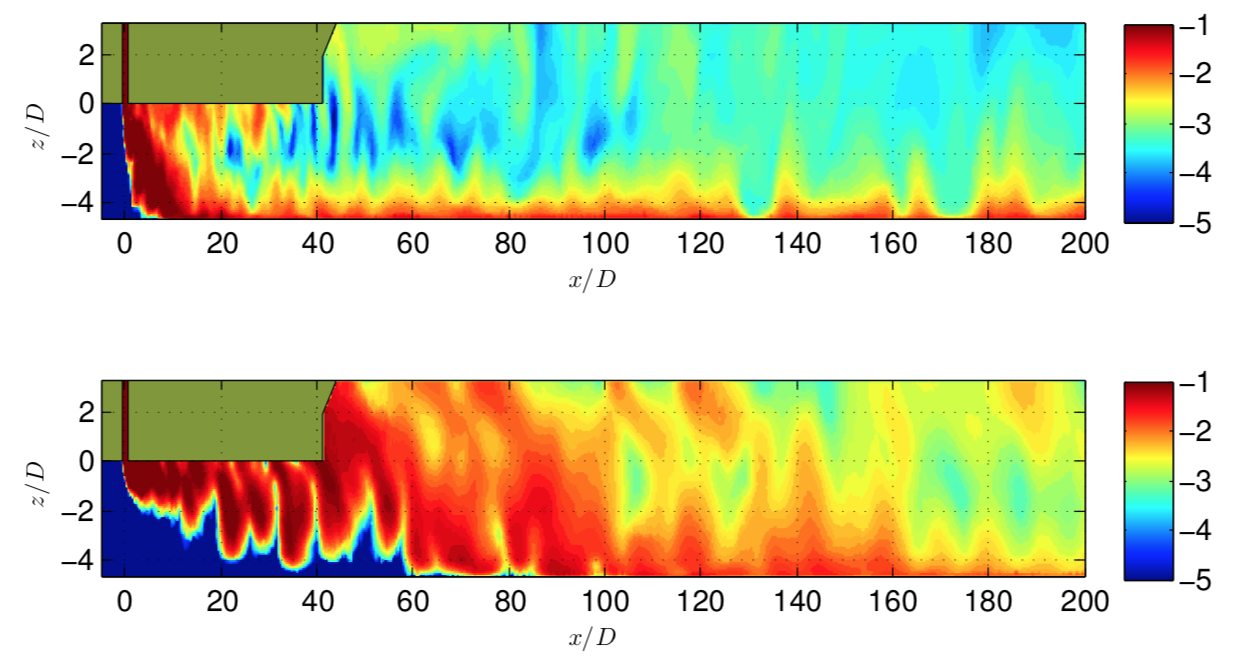
\includegraphics[width = .8\linewidth]{Images/dreding_speed.png}
    \caption{Contours of log C/$C_0$. Top panel: $U_{cf}$ =  1 m/s , lower panel: $U_{cf}$ =  3 m/s}
    \label{fig:dredging_speed}
\end{figure}

\noindent In the second case, the speed through water was increased to $U_{cf}$ = 3 m/s. For example, this situation occurs while trailing with speed over ground of 2 m/s in a current velocity of 1 m/s, head on. The resulting plume is shown in figure \ref{fig:dredging_speed}, lower panel. It is shown that due to the increased $U_{cf}$, a large part of the plume is lifted enough to be caught by the propellers. As a result, a much higher amount of sediment is mixed towards the surface. The sediment concentration in the surface plume is c/$C_0$ =  $10^{-2.5}$ at x/D = 100. A threefold increase in $U_{cf}$ has therefore resulted in a tenfold increase in the surface plume concentration. \newline

\noindent \cite{Dewit} did a comparable experiment to see what dredging speed did to the plume contours underwater. Instead of determining a $U_{cf}$ value, the jet-to-cross flow velocity ratio is determined. A value of $\lambda$ =  1.28 was chosen for normal dredging speed and a value of $\lambda$ =  0.68 for high dredging speed. As figure \ref{fig:dredging_speed_2} describes the two cases, a decrease in jet-to-cross flow velocity ratio clearly increases the surface plume in the near field.

\begin{figure}[ht!]
    \centering
    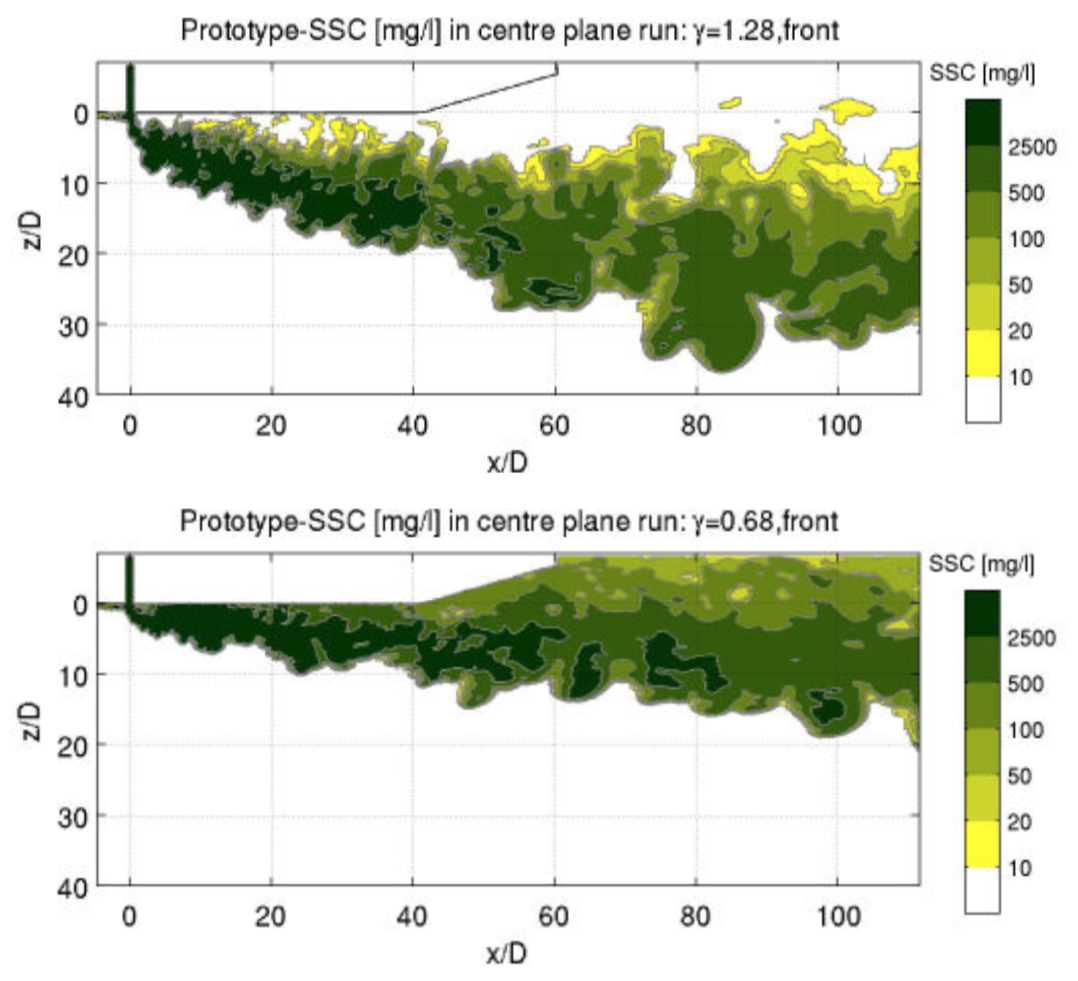
\includegraphics[width = .6\linewidth]{Images/Dredging_speed.png}
    \caption{SSC with normal dredging speed ($\lambda$ = 1.28) and high dredging speed ($\lambda$ = 0.68)}
    \label{fig:dredging_speed_2}
\end{figure}

\noindent In addition, as can be seen from figure \ref{fig:dredging_speed_3}, a difference in horizontal spreading is visible. A high dredging speed will decrease the horizontal spreading of the plume with a more dense packed plume \citep{Dewit}.

\begin{figure}[ht!]
    \centering
    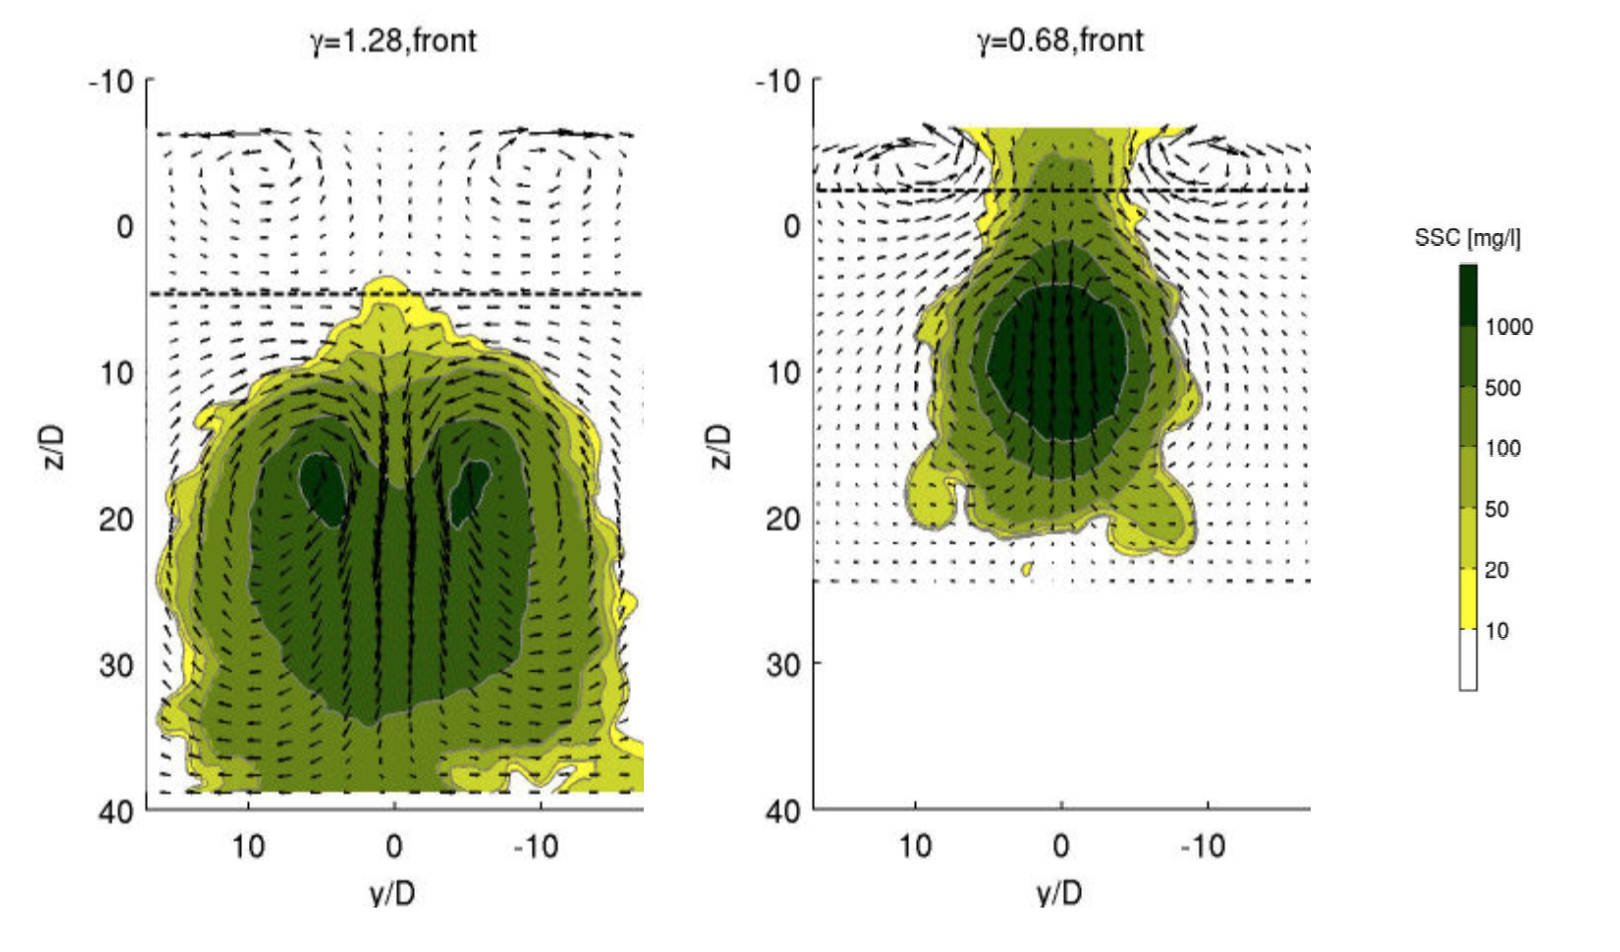
\includegraphics[width = .8\linewidth]{Images/Dredging_Speed_width.png}
    \caption{SSC at x = 100D with normal dredging speed (left) and high dredging speed (right)}
    \label{fig:dredging_speed_3}
\end{figure}











%%%%%%%%%%%%%%%%%%%%%%%%%%%%%%%%%%%%%%%%%%%%%%%%%%%%%%%%%%%%%%%%%%%%%%%%%%%%%%%%%%%%%%%%%%%%%%%%%%%%%%%%%%%%%%%%%%%%%%%%%%%%%%%%%%%%%%%%%%%%%%%%%%%%%%%%%%%%


\nomenclature[A]{$H_k$}{Depth below the keel \nomunit{[-]}}
\nomenclature[Z]{VIF}{Vertical Distribution of flux of fines}

\section{Dredging / water depth}

In figure \ref{fig:depth_belg}, vertical profiles of $C$/$C_0$ are given at y = 0 and x/D = 100 and horizontal profiles are shown in the surface plume at y = 0 and at 0.5m below the surface. It can be observed that the case with keel clearance ($H_k$) of 5m differs substantially from the other cases. The sediment concentration in the surface plume is about 4 times higher at x/D = 100. In the horizontal profile, the concentrations are similar for the cases with $H_k$ $\geq$ 9m, but for $H_k$ = 5m the surface concentration increases significantly at about x/D = 60. This location is at 30-40m behind the propellers \citep{Decrop}. Concluding figure \ref{fig:depth_belg}, water depth does influence the sediment concentration in suspension for $H_k$ $\geq$ 9m, but does not influence the sediment concentration at the water surface.

\begin{figure}[ht!]
    \centering
    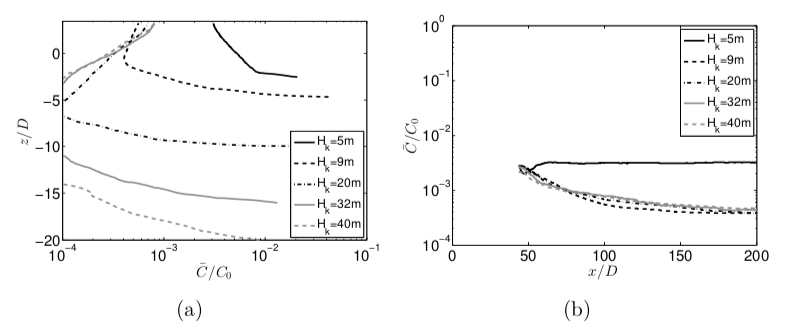
\includegraphics[width = 0.9\textwidth]{Images/depth_belg.png}
    \caption{Time-averaged sediment concentration $C$/$C_0$, for identical cases except for the different keel clearance $H_k$. In figure (a), vertical profiles are given at y = 0 and x/D = 100. In figure (b), horizontal profiles are given at y = 0 and at 0.5m below the surface.}
    \label{fig:depth_belg}
\end{figure}

\noindent In figure \ref{fig:depth_belg_2}, the streamwise velocity at y = 0 is shown for two keel heights calculated by the LES model of \cite{Decrop}. The difference in streamwise velocity is very noticeable where with decreasing water depth, the streamwise velocity distribution becomes less broad, with large areas with higher velocities.

\begin{figure}[ht!]
    \centering
    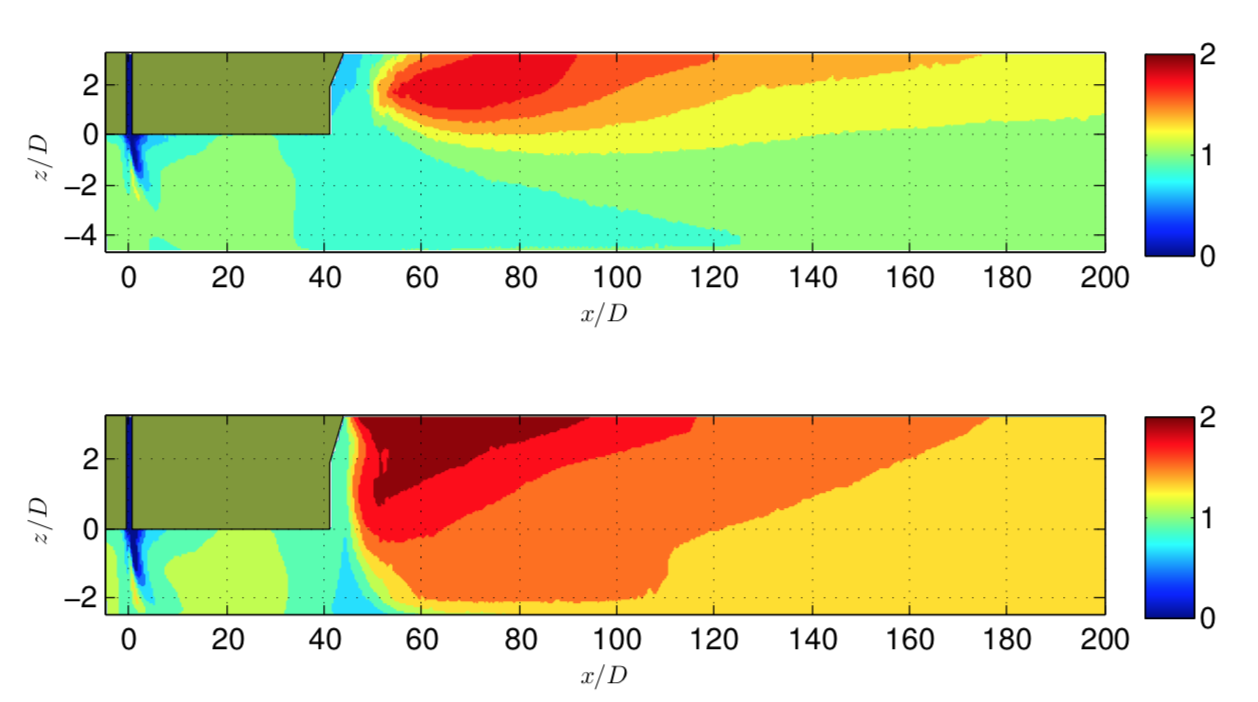
\includegraphics[width = 0.9\textwidth]{Images/depth_velocity_belg.png}
    \caption{Time averaged streamwise velocity at y = 0. top: $H_k$ = 9m, bottom: $H_k$ = 5m}
    \label{fig:depth_belg_2}
\end{figure}



\newpage
\noindent \cite{Dewit} calculated the vertical distribution of flux of fines in suspension (figure \ref{fig:depth_dewit}) to illustrate the effects of near field conditions like dredging speed, water depth, pulsing and air entrainment. All vertical distributions for situations with low $U_{cf}$ and large depth are strongly concave with the majority of the flux near the bed. For runs with large $U_{cf}$ or smaller depth the curves are less concave. For the smallest depth = 12m all curves are near linear, independent of air, pulsing or $U_{cf}$. A linear curve indicates a vertically fully mixed plume. The cases with lower density show a higher vertical distribution comparing to the higher density, which indicates that more particles found higher in the water column which makes sense with a lower density. \newline \noindent 

\begin{figure}[ht!]
    \centering
    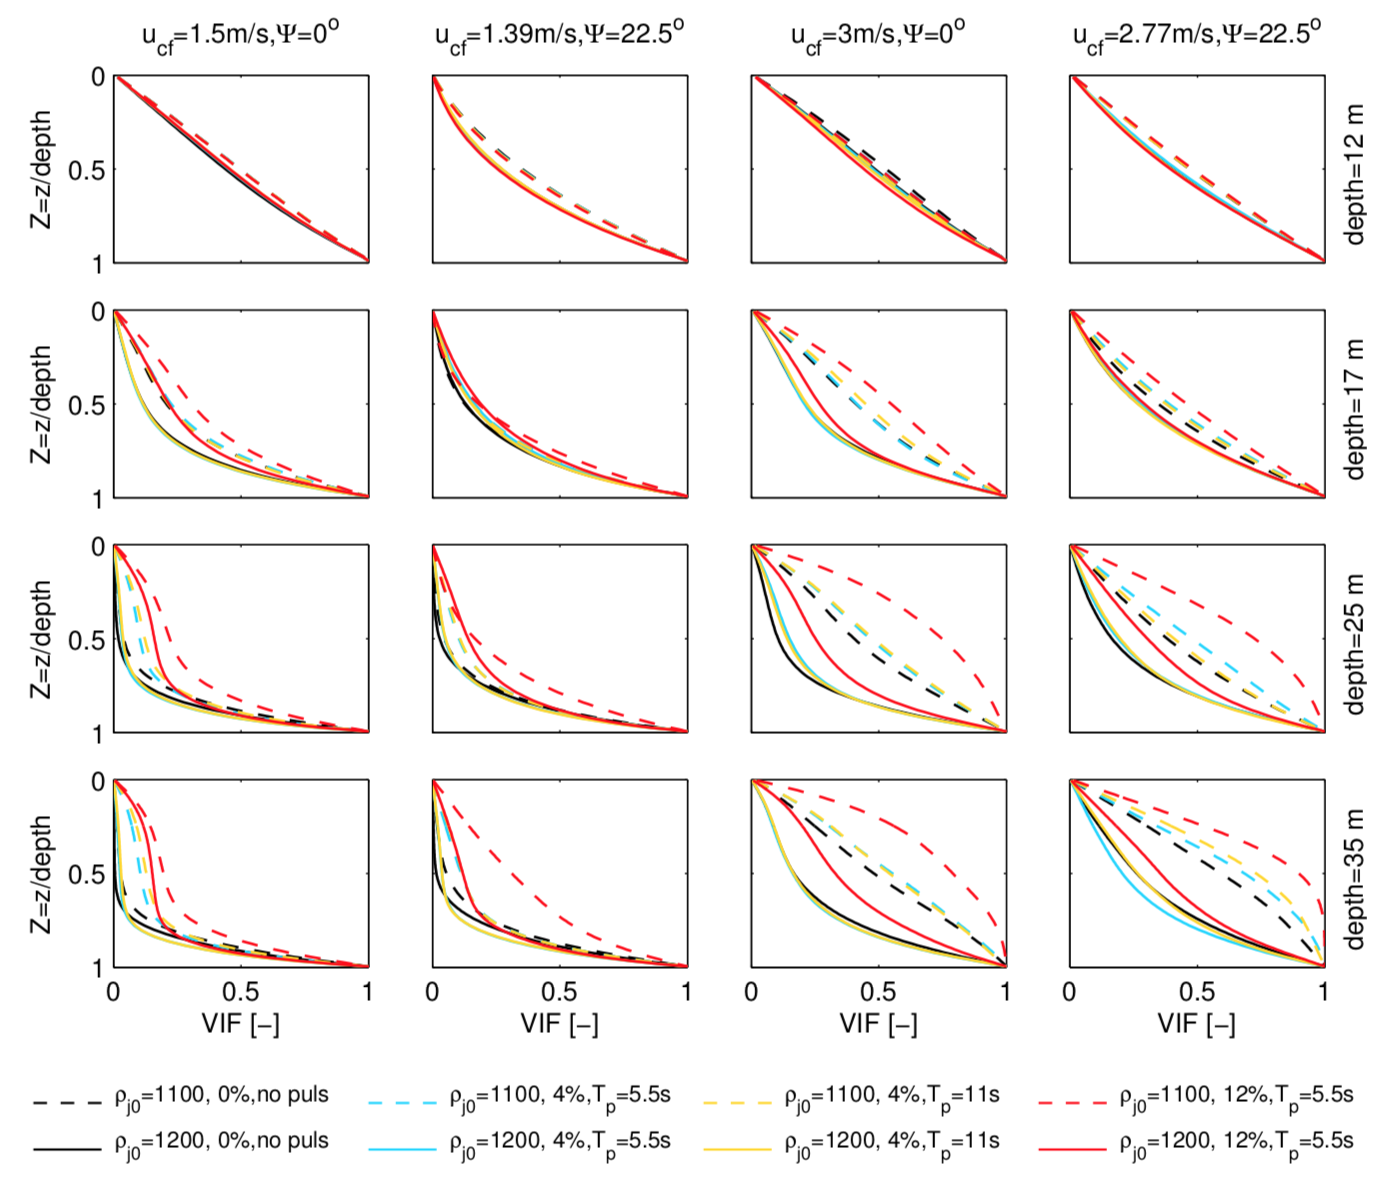
\includegraphics[width = 1\textwidth]{Images/Dredging_depth.png}
    \caption{Vertical distribution of the flux of fines (VIF =  $\int_{0}^{Z}$ 0Z flux dZ / $\int_{0}^{1}$ flux dZ, with Z =  z/depth) at the end of near field x =  350m}
    \label{fig:depth_dewit}
\end{figure}










%%%%%%%%%%%%%%%%%%%%%%%%%%%%%%%%%%%%%%%%%%%%%%%%%%%%%%%%%%%%%%%%%%%%%%%%%%%%%%%%%%%%%%%%%%%%%%%%%%%%%%%%%%%%%%%%%%%%%%%%%%%%%%%%%%%%%%%%%%%%%%%%%%%%%%%%%%%%
\newpage
\section{Angle between TSHD and ambient current}

A high cross flow velocity leads to a larger plume flux still in suspension after a certain settling time, more sediment in higher parts of the water column and thus a large surface plume. A high cross flow velocity increases the interaction between the plume and the TSHD hull and the plume and the TSHD propellers. When a TSHD is sailing under an angle with the ambient current, the overflow plume is pushed towards the side of the TSHD hull where it can be taken along by the expanding flow towards the free surface. The more the ambient current comes from the side, the more surface plume can be expected\citep{Dewit}. When looking at figure \ref{fig:depth_dewit}, dredging under an angle $\psi$ =  22.5$^\circ$ to the ambient velocity gives lifted vertical distribution profiles with more material in the upper parts of the water column than for $\psi$ =  0$^\circ$. The one exception is the case with depth =  12m where $U_{cf}$ =  1.39m/s, $\psi$ =  22.5$^\circ$ has a lower vertical distribution profile than $U_{cf}$ = 1.5m/s, $\psi$ = 0$^\circ$.

\begin{figure}[ht!]
    \centering
    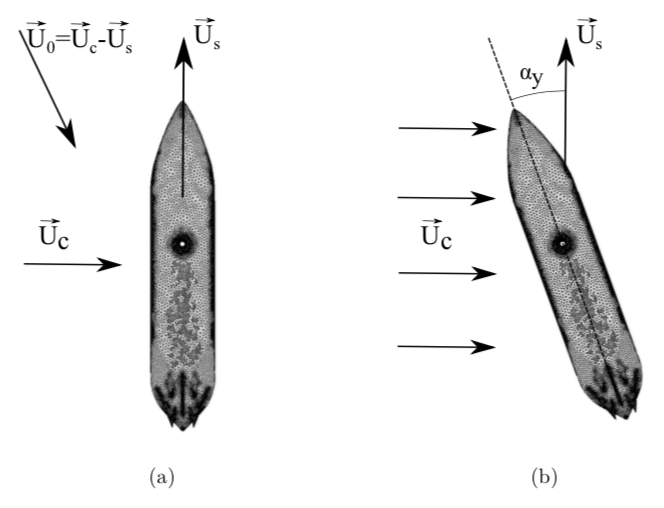
\includegraphics[width = .6\linewidth]{Images/Anlge_TSHD.png}
    \caption{(a) Modeling approach for a ship in a cross current: the through-water velocity $U_0$ is equal to the cross current velocity vector $U_c$ minus the ship’s course vector $U_s$. (b) Definition of the yaw angle $\alpha_y$ of a ship sailing in a cross current.
}
    \label{fig:Angle_TSHD}
\end{figure}


\noindent \cite{Decrop} simulated a TSHD sailed at $U_s$ = 0.9 m/s (over ground) in a perpendicular cross current of $U_c$ = 0.45 m/s. See figure \ref{fig:Angle_TSHD}a for a sketch. This results in a net speed through water of $U_{0}$ = 1 m/s and an angle between the ship center line and its speed through water of $\psi$ = 26.6$^\circ$. In the LES model, the ship is considered stationary with its center line along the x-axis and the net current is imposed at the boundary. The angle of 26.6$^\circ$ is, however, an overestimation. Indeed, for a ship to follow its course in a cross current, it must develop some yaw angle. A ship’s yaw angle is the angle between the course and the vessel center line (figure \ref{fig:Angle_TSHD}b). When a ship is sailing in a cross current, its yaw angle or drifting angle $\alpha_y$ is estimated by \cite{Pianc}.

\nomenclature[A]{$U_0$}{Ambient cross flow velocity \nomunit{[$m/s$]}}

\begin{equation}
    tan (\alpha_y) =  \frac{U_c}{U_s}
\end{equation}


\noindent This equation returns exactly the same angle as initially found for the angle between the ship center line and the velocity vector relative to the water, $U_0$. This means a ship would always align itself with the relative velocity $U_0$. A TSHD with drag head on the sea bed has some kind of anchoring, due to which $\alpha_y$ might be smaller than atan(Uc/Us). However, setting the angle $\alpha$ simply to atan($U_c$/$U_s$) is not correct. The angle between a ship and its speed through water will be much lower. In this sense, the simulation with $\psi$ = 26.6°corresponds with a situation with a cross flow significantly stronger than 0.45 m/s, or with an anchored TSHD serving as a barge for cutter dredgers. The other plume boundary conditions were set to $C_0$ = 55 g/l and $W_0$ = 1.9 m/s. \newline \newline
\noindent When looking at the time-averaged $C$/$C_0$ in a cross section (x/D = 50), it can be observed that the plume is asymmetric (figure \ref{fig:Angle_TSHD2}, top panel). It can be seen that the surface plume is situated around y/D = 15 at x/D = 50. The angle of the path of the surface plume is therefore about atan(15/50) = 16.7°. This is lower than the angle between the ship and the relative velocity $U_0$. The near-bed density current is positioned around y/D = 30, corresponding to a path angle of atan(30/50) = 31°. This is larger than the angle of the relative velocity $U_0$. The density current and the surface plume clearly feel the influence of the cross current in a different way. In order to analyze this situation, a detailed three-dimensional visualization is needed.
The resulting surface plume and subsurface density current are shown in figure \ref{fig:Angle_TSHD2}, lower panel. It can be seen that the density current follows another angle compared to the surface plume. The descending density current feels a secondary current induced by the angle between ship and flow. Therefore the density current is diverted towards a higher angle than the cross flow (towards the left of the figure).

\begin{figure}[ht!]
    \centering
    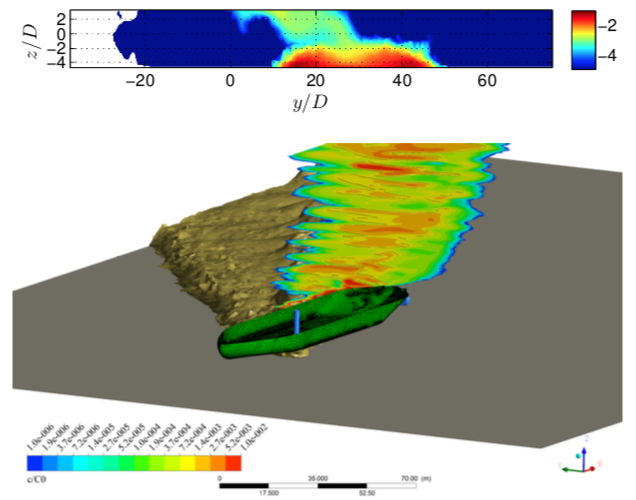
\includegraphics[width = .7\linewidth]{Images/Angle_TSHD2.png}
    \caption{TSHD sailing in a cross flow. Top panel: Vertical cross section of time-averaged sediment concentration field log($C$/$C_0$) at x/D = 50. Lower panel: Surface plume concentration $c$/$C_0$ in colour scale and density current in brown iso-surface.
}
    \label{fig:Angle_TSHD2}
\end{figure}

\noindent The question is now whether the surface plume in a cross flow has significantly different concentration levels as compared to a plume without cross flow. In figure \ref{fig:Angle_TSHD3}, the instantaneous concentration log($C$/$C_0$) for a plume without cross flow and for the same plume with a cross flow is shown. The concentration levels in the surface plumes are very similar. The surface plume in the cross flow case is wider and has a larger variation in $C$. It can be calculated, however, that the total sediment flux in both plumes is quite similar \citep{Decrop}. But as can be seen in figure \ref{fig:Angle_TSHD3}b, a higher concentration at the surface can be seen at higher x/D values compared to no cross flow like in figure \ref{fig:Angle_TSHD3}a. A diverted flow will interact with the hull, where a flow towards the surface is present due to the movement of the vessel. Sediment can be taken along with this flow, which will increase the surface plume \citep{Dewit}.


\begin{figure}[ht!]
    \centering
    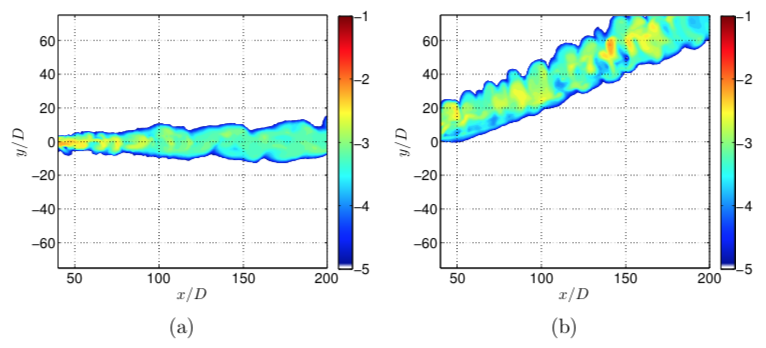
\includegraphics[width = .75\linewidth]{Images/Angle_TSHD3.png}
    \caption{Instantaneous concentration log($c$/$C_0$) for a plume without cross flow (a) and for the same plume with a cross flow (b).
}
    \label{fig:Angle_TSHD3}
\end{figure}










%%%%%%%%%%%%%%%%%%%%%%%%%%%%%%%%%%%%%%%%%%%%%%%%%%%%%%%%%%%%%%%%%%%%%%%%%%%%%%%%%%%%%%%%%%%%%%%%%%%%%%%%%%%%%%%%%%%%%%%%%%%%%%%%%%%%%%%%%%%%%%%%%%%%%%%%


\nomenclature[Z]{SSC}{Suspended Sediment Concentration}
\nomenclature[A]{$St$}{Strouhal number \nomunit{[-]}}
\nomenclature[A]{$T_p$}{Pulsing period \nomunit{[$s$]}}


\section{Pulsing}
A pulsing, discontinuous flow (also shortly treated in section \ref{sec:plume}) in the overflow has been measured on a field trip \citep{Dewit}. The pulsing frequency is dependent on the ambient wave period and the dynamic motions of the TSHD. Pulsing has two effects on the dredging plume: it enhances vertical spreading of the plume and it gives a deeper plume path. The deeper plume path is caused by the extra initial inflow momentum compared to a continuous non-pulsed case with similar volume flux. Pulsing can either enhance the formation of a surface plume by the increased vertical spreading or reduce the formation of a surface plume by the deeper plume path which reduces the influence of the TSHD hull and propellers. For a high cross flow velocity it is found that pulsing results in a smaller surface plume and for a low cross flow velocity pulsing results in a larger surface plume \citep{Dewit}. \newline 
\noindent \cite{Dewit} used a pulsing period ($T_p$) based on a frequency in the range of the Strouhal number ($fD / U_0$) to determine the fluctuation inflow of the overflow. Figure \ref{fig:pulsing} shows three cases with different pulsing periods depending on the Strouhal number. Where a St = 0.27 describes the smallest pulsing period, St = 0.18 describes the middle pulsing period and St = 0.12 describes the largest pulsing period. \newline

\begin{figure}[ht!]
    \centering
    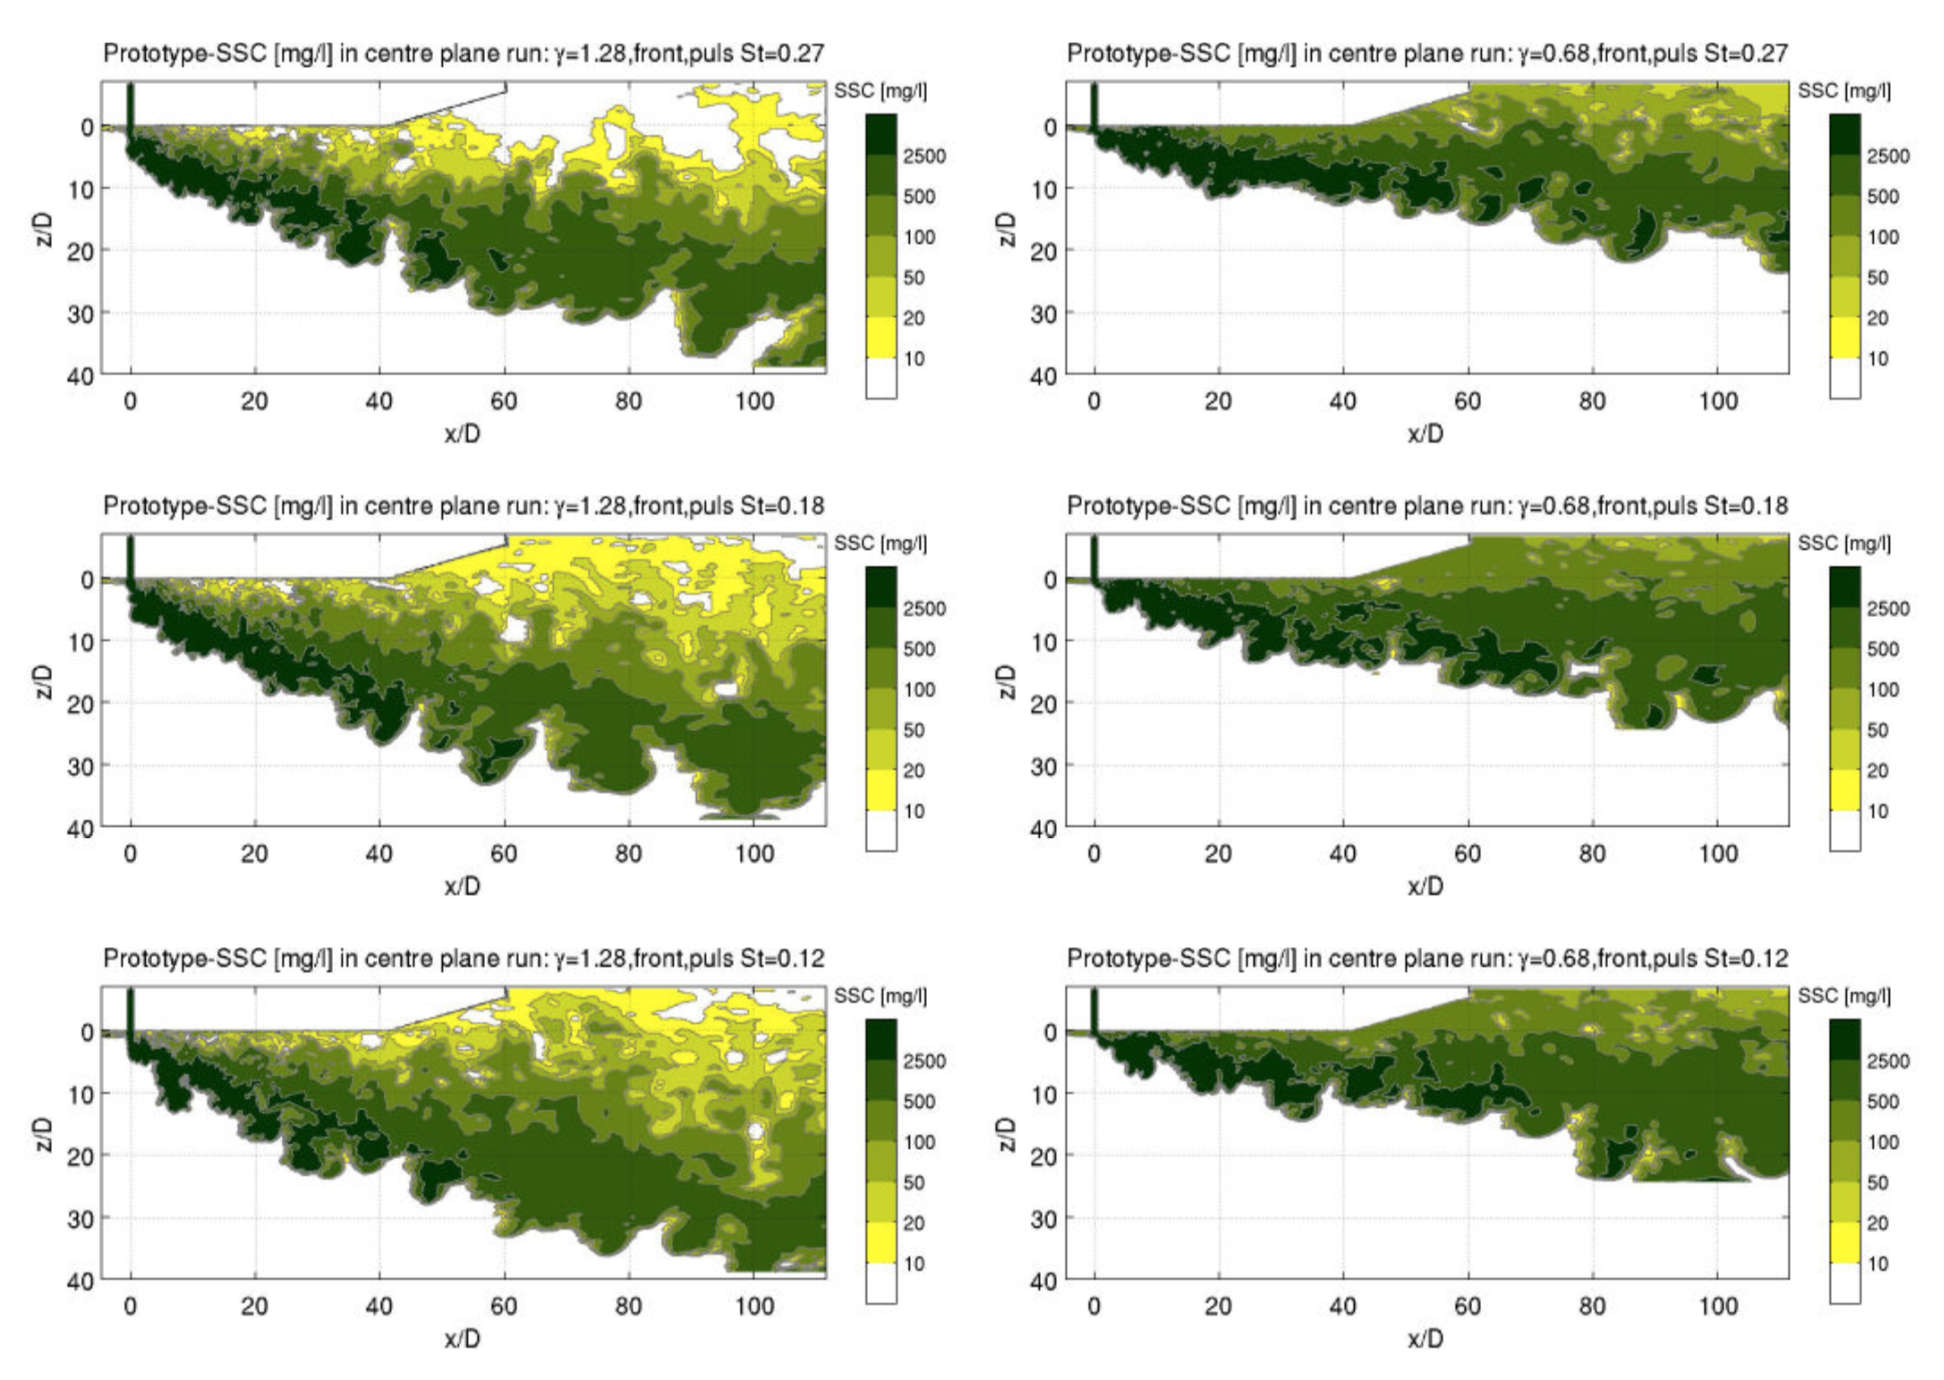
\includegraphics[width = 1\textwidth]{Images/Pulsing.png}
    \caption{SSC with pulsing}
    \label{fig:pulsing}
\end{figure}

\nomenclature[G]{$\lambda$}{Jet-to-cross flow velocity ratio \nomunit{[-]}}

\noindent Figure \ref{fig:pulsing} describes the effect of pulsing on the SSC near field. The left figures describe a normal dredging speed were the right figures describe a high dredging speed and so low $\lambda$ value. As can be seen of the three right figures, the pulsing period does not have a large effect with a high dredging speed: a significant surface plume is visible. Looking at the normal dredging speed, the pulsing period does have a large influence on the SSC. For the largest pulsing period, the separate puffs including gaps can be recognized. More general, a larger pulsing period increases the surface plume. \newline \noindent
When looking at figure \ref{fig:depth_dewit}, air with pulsing lifts the vertical distribution profile up with a small effect of 4\% with $T_p$ =  5.5s or $T_p$ =  11s pulsing and a big effect of 12\% air with $T_p$ =  5.5s. The runs with depth = 25m or 35m, $\rho_{j0}$ =  1100kg/m3 and 12\% air with pulsing even show convex curves: more than 50\% of the fines flux still in suspension can be found in the upper half of the water column and the plume is floating above the bed without touching it \citep{Dewit}.










%%%%%%%%%%%%%%%%%%%%%%%%%%%%%%%%%%%%%%%%%%%%%%%%%%%%%%%%%%%%%%%%%%%%%%%%%%%%%%%%%%%%%%%%%%%%%%%%%%%%%%%%%%%%%%%%%%%%%%%%%%%%%%%%%%%%%%%%%%%%%%%%%%%%%%%%

\nomenclature[Z]{LPM}{Liters Per Minute}
\section{Air}
\label{sec:air}
When the water level inside the vertical overflow shaft is much lower than the water level inside the hopper, the overflowing water forms a plunging jet in the shaft and significant amounts of air can be entrained into the overflow plume. So, the air entrainment and pulsing of the overflow are closely related. There is experimental evidence that a main plume and the air content of this plume will separate into two separate plumes at a certain distance from the source \citep{Zhang+}. The experimental setup is shown in figure \ref{fig:Zhang_experiment}.

\begin{figure}[ht!]
    \centering
    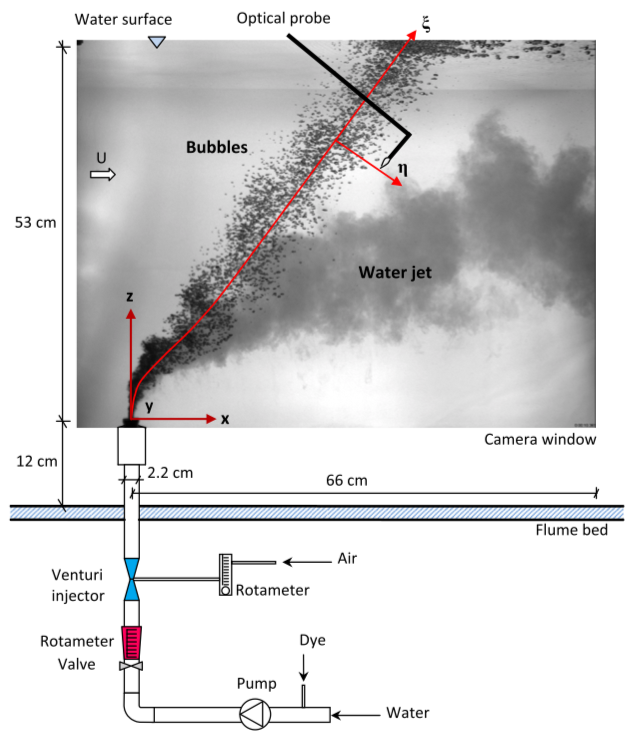
\includegraphics[width = 0.5\textwidth]{Images/Zhang_experiment.png}
    \caption{Schematic side view of the experimental setup (the optical probe drawn in a larger scale), with indication of coordinate system and camera window}
    \label{fig:Zhang_experiment}
\end{figure}
\noindent
In this study, a total of 12 experimental scenarios were investigated (see figure \ref{fig:Zhang_experiment_2}): the air flow rate $Q_a$ at the nozzle was set to be 1, 3 and 5LPM; and the water flow rate $Q_w$ was 0, 1, 3 and 5LPM. Experiments are identified with two numbers: the first and second number are for $Q_a$ and the $Q_w$, respectively. To visualize the trajectories of the liquid-phase in bubbly jets, dye was injected into the water pipeline upstream of the water pump \citep{Zhang+}. 


\begin{figure}[ht!]
    \centering
    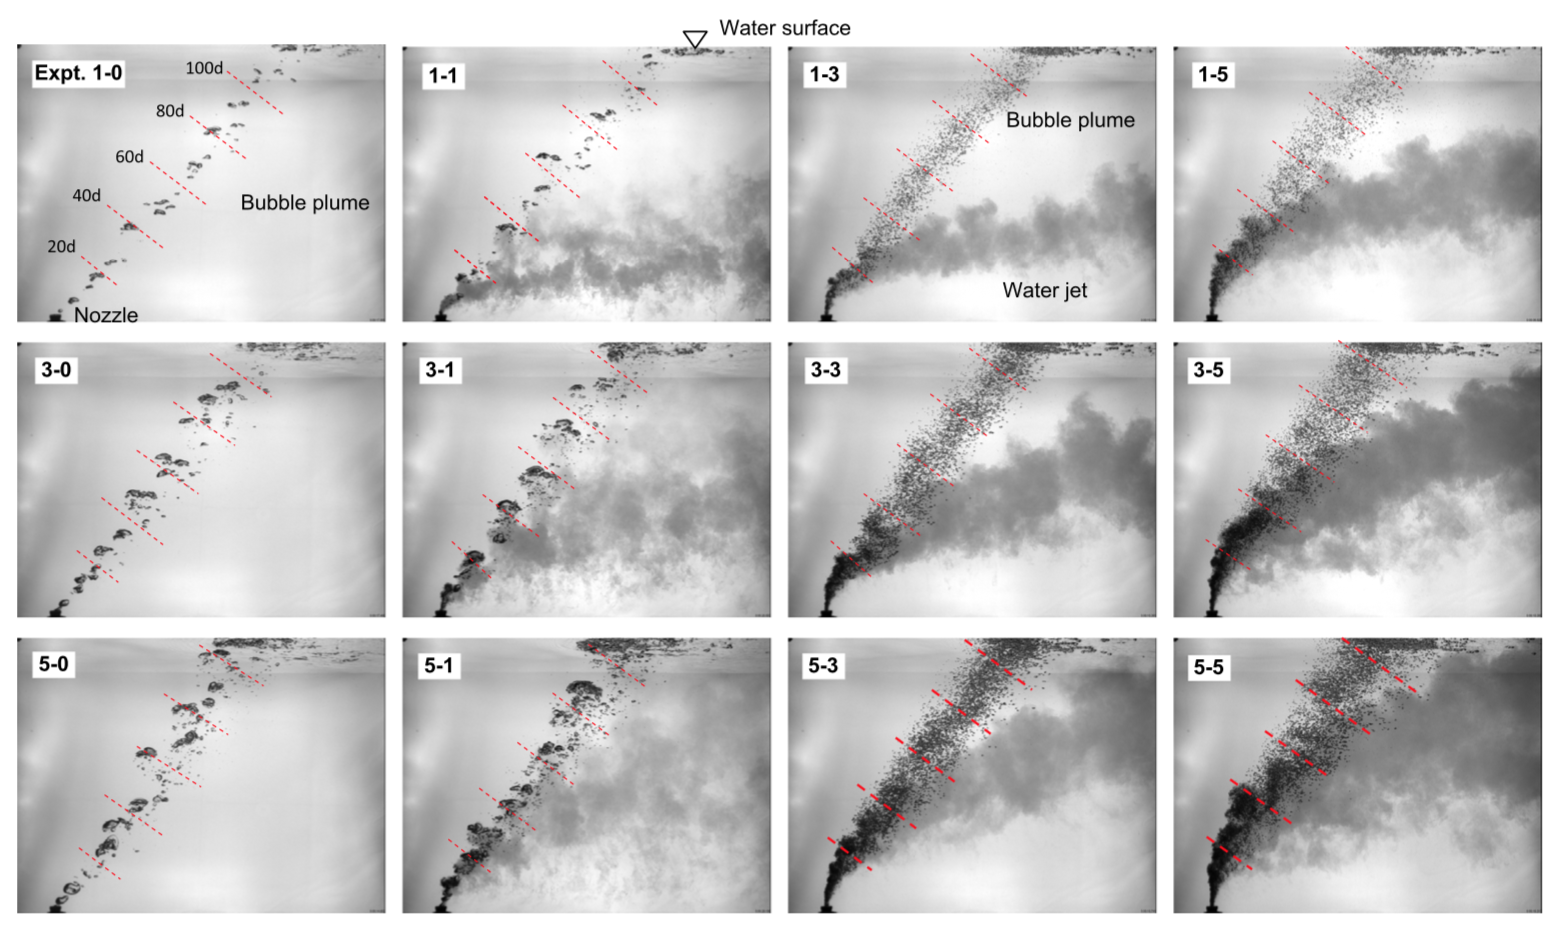
\includegraphics[width = 1\textwidth]{Images/Zhang_experiment_2.png}
    \caption{Photos of bubbly jets in 12 experimental conditions; side view, the first and second numbers in the experiment scenarios represent the air and water discharges at the nozzle (unit: LPM), respectively}
    \label{fig:Zhang_experiment_2}
\end{figure}
\newpage
\noindent As clearly can be seen, when a mixed jet with both air- and water discharge is injected, the jet splits in a clear air path and water path. The separation height appears to increase with the increase in $Q_a$ or $Q_w$, e.g., it increases from approximately section 20d in experiment 1–3 to section 40d in experiment 3–3 and further to Section 60d in experiment 5–3; and it increases from below section 20d in experiment 1–1 to section 20d in experiment 1–3 and further to section 40d in experiment 1–5. The increase of separation height can be explained by the increase of the liquid jet momentum at the nozzle exit \citep{Zhang+}. \newline

\noindent Connecting this to dredging on a TSHD with overflow losses, the influence of air creates a uprising buoyant flow to the water surface which can pick up fine particles and so create a surface plume. Under the influence of gravity, air bubbles are rising, which can be seen as a negative (upward) settling velocity. The terminal rising velocity of air bubbles is reached when buoyancy and drag reach equilibrium. The relation between the terminal air bubble rise velocity and air bubble diameter for still water from \cite{Clift+} for fresh water and from \cite{Chanson+} for fresh water and sea water are presented in figure \ref{fig:bubble_rise}.

\begin{figure}[ht!]
    \centering
    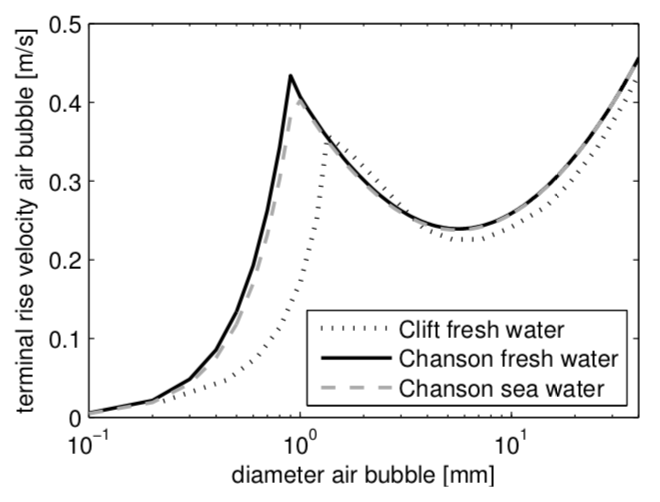
\includegraphics[width = 0.5\textwidth]{Images/bubble_rise.png}
    \caption{Terminal air bubble rise velocity in 20$^{\circ}$C water}
    \label{fig:bubble_rise}
\end{figure}

\noindent The difference between the air bubble rise velocity in fresh water and in sea water for similar bubble diameter is negligible. However, air bubbles created at a plunging jet in sea water are finer than in fresh water, air bubble fusion is reduced and less air volume is entrained: in a scale experiment of a plunging jet with a nozzle diameter of 12.5 mm \cite{Chanson2006+} found a wide variety in air bubbles chord lengths of < 0.5 mm to > 10 mm for fresh and sea water with a smaller mean air bubble chord length in sea water of 3 to 6 mm compared to the mean air bubble chord length of 4 to 7 mm in fresh water. \newline 
\noindent The smaller air bubble size and lower air volume entrainment in sea water can partly be explained by physical properties as density, viscosity, salinity and surface tension, but these physical properties cannot explain all observed differences. Sea water also gives less air entrainment and smaller bubble sizes than saline water, therefore additional differences as organic matter and living organisms (e.g. plankton, algae) must play a role as well \cite{Chanson2006+}. In a fresh water full scale experiment of a drop shaft with a drop height of 1.7 m, bubble chord sizes of <0.5 to >25 mm are measured with mean values of 8 to 10 mm in the drop shaft below the water line and mean values of 2 to 5 mm in the horizontal outflow channel \citep{Chanson}. \newline
The overflow of a TSHD is a sand-mud-water mixture drop shaft with drop heights in the order of 0 to 3 m. Dredging often takes place at sea, therefore smaller air bubble sizes are expected than in the experiment of \cite{Chanson} with fresh water. Based on the results of \cite{Chanson2006+} and \cite{Chanson} air bubbles in the overflow are expected to have diameters of <0.5 to >25 mm with a mean diameter in the range of 1 to 9 mm. The sea water air bubble rise velocity for bubble sizes of 1 to 9 mm is 0.4 to 0.24 m/s. \newline

\noindent \cite{Dewit} used these references in his LES model. Figure \ref{fig:air_dewit} shows the difference between 0\% air entrainment (left figure) and 12\% air entrainment with $T_p$ = 5.5s (right figure) at x = 350m, what is declared as the end of the near field of the model. 

\begin{figure}[ht!]
    \centering
    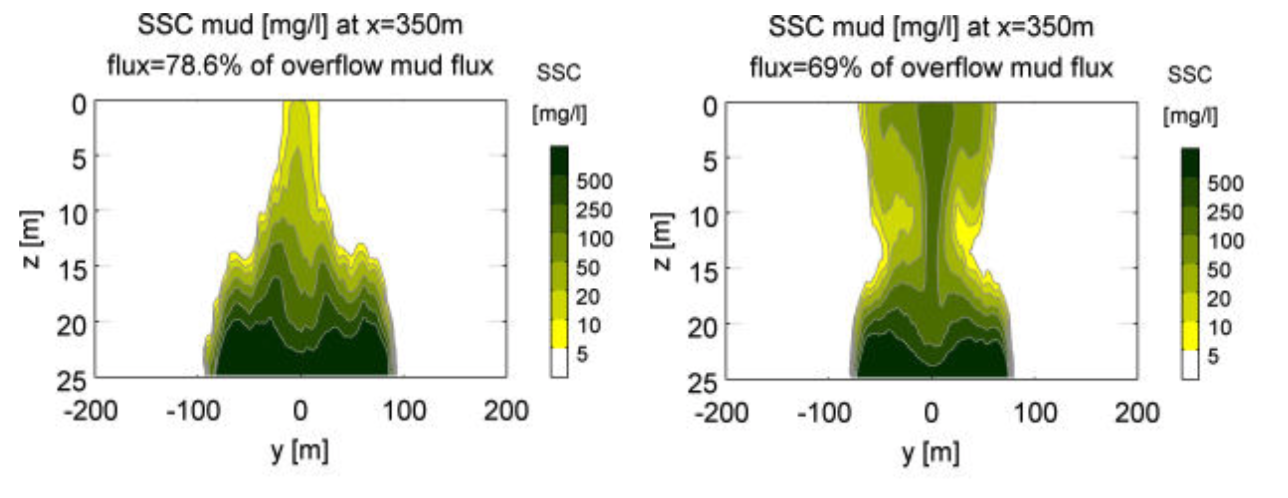
\includegraphics[width = 0.8\textwidth]{Images/air_0_12.png}
    \caption{Simulated result at end near field x =  350m from \cite{Dewit} with left: 0\% air entrainment, right: 12\% air entrainment with $T_p$ = 5.5s}
    \label{fig:air_dewit}
\end{figure}

\noindent The influence of entrained air is conditional, largest influence is found with a low cross flow velocity combined with a large depth. With high cross flow velocity and/or small depth a big surface plume with high turbidity at the free surface can be found, independent of the amount of entrained air \citep{Dewit}. \newline

\noindent \cite{Decrop} tested the effect of the air bubble reduction, by comparing the simulation with- and without air reduction for two cases: a high plume case and a case with plume sediment mixed throughout the water column based on information form \cite{Saremi+}. In figure \ref{fig:air_belg}, the results are shown in terms of vertical sediment concentration profiles at the plume centerline. In the case with deep water and a high plume trajectory (figure \ref{fig:air_belg}a), the effect of decreasing the air entrainment with 90\% is clear. The concentration near the surface is reduced drastically, around a factor 20, which can be explained by the absence of the vertical momentum source in the water-sediment mixture due to the wakes of the rising air bubbles (eq. \ref{eq:bulk}).

\begin{figure}[ht!]
    \centering
    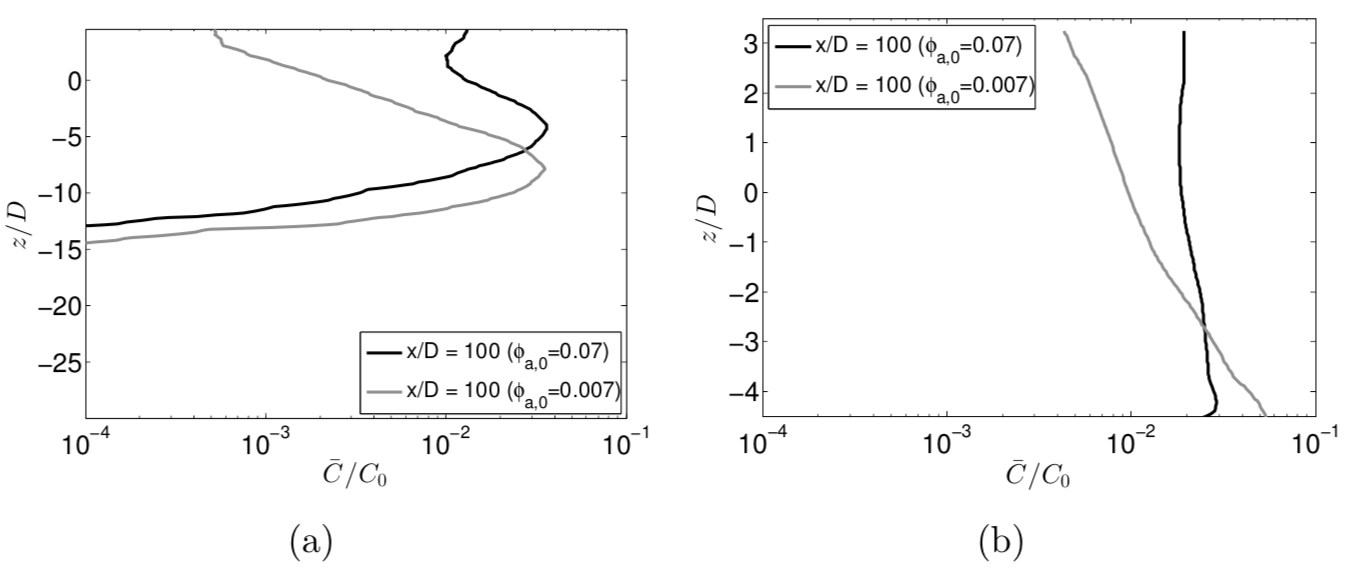
\includegraphics[width = 0.8\textwidth]{Images/air_belg.png}
    \caption{Profiles of time-averaged sediment concentration $C$/$C_0$ for a case with high trajectory (a) and a case with mixed sediments (b). For each case, a simulation is run with a regular initial air bubble volume fraction ($\phi_{a,0}$ = 7\%) and with a 90\% reduction of $\phi_{a,0}$ = 0.7\%}
    \label{fig:air_belg}
\end{figure}

\noindent It is noticed that the bulk of the plume is situated deeper with a reduced air concentration. This effect is simply explained by the increased bulk density of the plume when the air volume fraction is lower. The bulk mass density of the water-sediment-air mixture is defined by:

\begin{equation}
\centering
    \rho_m =  (1-\phi_s-\phi_a)\rho_w + \phi_s\rho_s + \phi_a\rho_a 
    \label{eq:bulk}    
\end{equation}

\noindent where $\phi_s$ and $\phi_a$ are the volume fractions of sediment and air and $\rho_m$, $\rho_s$, $\rho_w$ and $\rho_a$ are the mass densities of respectively the mixture, the sediment, sea water and air. It can be shown that for an air fraction of 7\%, mixtures with $C_0$ up to 13 g/l have a positive buoyancy, which means they are lighter than the surrounding sea water and will flow up to the water surface. For $\phi_a$ = 14\% this is even the case up to $C_0$ = 26 g/l \citep{Decrop}. \newline


\nomenclature[G]{$\rho_a$}{Mass density of air \nomunit{[$kg/m^3$]}}
\nomenclature[G]{$\rho_m$}{Mass density of mixture \nomunit{[$kg/m^3$]}}
\nomenclature[G]{$\phi_s$}{Volume fraction of sediment \nomunit{[-]}}
\nomenclature[G]{$\phi_a$}{Volume fraction of air \nomunit{[-]}}
\nomenclature[G]{$\alpha_y$}{Yaw angle \nomunit{$[^\circ]$}}
\nomenclature[G]{$\psi$}{Angle between the ship centerline and its speed through water \nomunit{$[^\circ]$}}

\noindent In the case with more shallow water and a near-bed density current combined with a surface plume, a different result is found (figure \ref{fig:air_belg}b). The bulk plume volume cannot descend deeper in the case with air reduction, since it is almost fully mixed throughout the water column. The surface concentrations, however, are also positively affected by the air reduction. It can be observed in the figure that with $\psi_{a,0}$ = 7\%, the sediment is mixed, while with $\psi_{a,0}$ = 0.7\%, the surface concentration is about five times lower than the near-bed concentration \citep{Decrop}. As can be seen, the air bubble reduction also has an effect on the plumes in more shallow water, however, it is four times more effective in deep water.













%%%%%%%%%%%%%%%%%%%%%%%%%%%%%%%%%%%%%%%%%%%%%%%%%%%%%%%%%%%%%%%%%%%%%%%%%%%%%%%%%%%%%%%%%%%%%%%%%%%%%%%%%%%%%%%%%%%%%%%%%%%%%%%%%%%%%%%%%%%%%%%%%%%%%%%%


\section{Interaction with propeller}
\label{sec:propeller}
%Belg 8.7.8 + figure 8.3.6
%De wit figuur 7.4

Whether the near-field overflow plume would be different without the propeller jet influence is of course a hypothetical question, no TSHD can sail without propellers. Nevertheless, it is interesting to see how the propeller influences the streamlines around the ship and how this in turn influences the (surface) plume. \newline \noindent Propellers create streamlines extending up- and downstream which show how the propeller jets evolve, see figure \ref{fig:Propeller_belg}. The tangential component of the propeller jet is only short-live: at a distance of 4D (propeller diameter), 90\% has dissipated \citep{Decrop}. 

\begin{figure}[ht!]
    \centering
    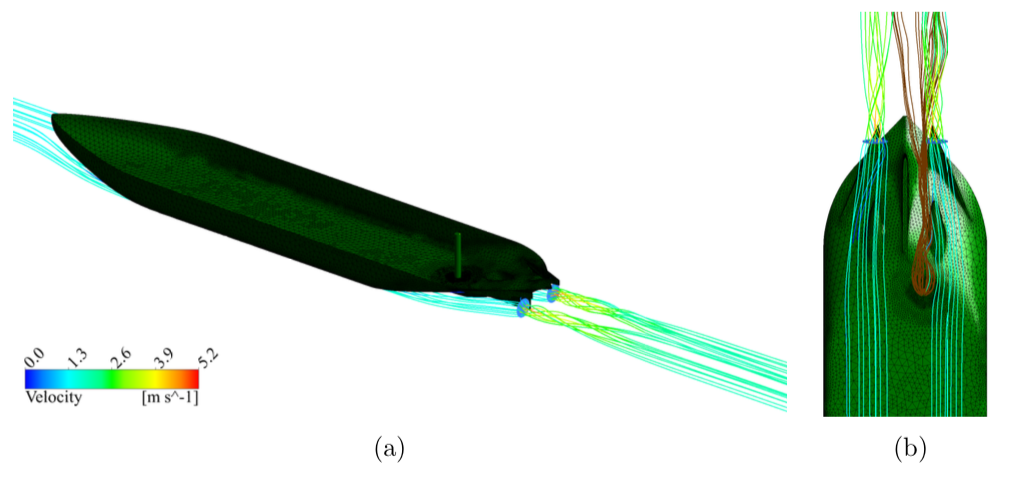
\includegraphics[width = 0.6\textwidth]{Images/Propeller_belg.png}
    \caption{Port side view of the streamlines going through the propellers (a). Bottom view of propeller streamlines and streamlines originating from an overflow with lateral shift of 5m from the centerline(b)}
    \label{fig:Propeller_belg}
\end{figure}

\noindent It can be seen that the propeller jet discharge originates from the keel, but not from the centerline of the keel. In the case of an overflow positioned along centerline of the ship, propeller streamlines do not go directly from overflow to propeller. In case of an overflow shifted from the centerline of the ship (figure \ref{fig:Propeller_belg}b), the sediment might go directly into the propellers.



\noindent The propellers also induce turbulent mixing. Following the gradient diffusion theory, turbulent mixing occurs in down-gradient direction. The vertical turbulent diffusion can be written as

\begin{equation}
    F_z =  -D_t \frac{\delta C}{\delta z}
    \label{eq:turbulent_diffusion}
\end{equation}

\noindent where $D_t$ is the turbulent diffusivity. \newline \newline \noindent
\cite{Decrop} visualized the vertical gradient of C before the plume arrives at the propeller influence. In this case, the propellers are at x/D = 40, but the influence of both propellers arrives at the centerline somewhat further. The propeller jets are located at a height of 0< z/D <3. Two cases can be distinguished: a case with $\delta C$/$\delta z$ <0 before arrival at the propellers and a case with $\delta C$/$\delta z$ >0 at the propeller. \newline 
\noindent In figure \ref{fig:Propeller_belg_2}a, a case is shown with $\delta C$/$\delta z$ <0 before arrival at the propellers (x/D = 30). At x/D = 50 not much influence is found yet. At x/D = 100, however, the effect of the propeller mixing is recognized. The negative vertical concentration gradient is flattened out due to turbulent mixing and thus results in an increase in the surface plume concentration. \newline 

\begin{figure}[ht!]
    \centering
    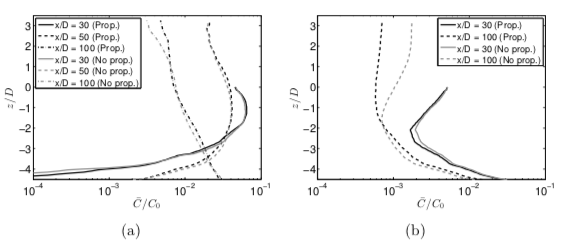
\includegraphics[width = 1\textwidth]{Images/Propeller_belg_2.png}
    \caption{Profiles of time-averaged sediment concentration $C$/$C_0$ for two plume cases: one with $\delta C$/$\delta z$ <0 near the keel and under the stern (a) and one with $\delta C$/$\delta z$ >0 at the same location (b). For each case, a simulation is run with and without propeller jets.}
    \label{fig:Propeller_belg_2}
\end{figure}

\noindent In figure \ref{fig:Propeller_belg_2}b, a case is shown with $\delta C$/$\delta z$ >0. The turbulent sediment flux is here expected to be downward and so the effect of the propeller is positive, particles will be transported downwards. Indeed, at x/D = 100, the sediment in the surface plume seems to be transported by the propeller jets to deeper parts, and the surface plume has a lower concentration. \newline 
\noindent It can be imagined that in most cases, $\delta C$/$\delta z$ might be smaller than zero since the plume emerges from under keel. However, the three-dimensional situation is more complex. The two propeller jets start away from the centerline, widen and meet the centerline after a certain distance. Over the course of this distance, the plume might have risen and $\delta C$/$\delta z$ might be larger than zero. This is again a case of coupled interaction between multiple parameters \citep{Decrop}. \newline

\noindent \cite{Dewit} used his model to look at the influence of a propeller with both normal- and high dredging speed (see figure \ref{fig:Propeller_dewit} for x-direction). It can be seen that a propeller has almost no influence when dredging at high speeds. At normal speeds, the propeller brings the plume up in the vertical. The influence in y-direction can be seen in figure \ref{fig:Overflow_position}. A propeller lifts the dredging plume up by entrainment into the propeller jet an this entrainment partly blocks the counter rotating vortex pair of the dredging plume. However, there is no indication that significant amounts of the dredging plume are sucked in directly into the propeller \citep{Dewit}.

\begin{figure}[ht!]
    \centering
    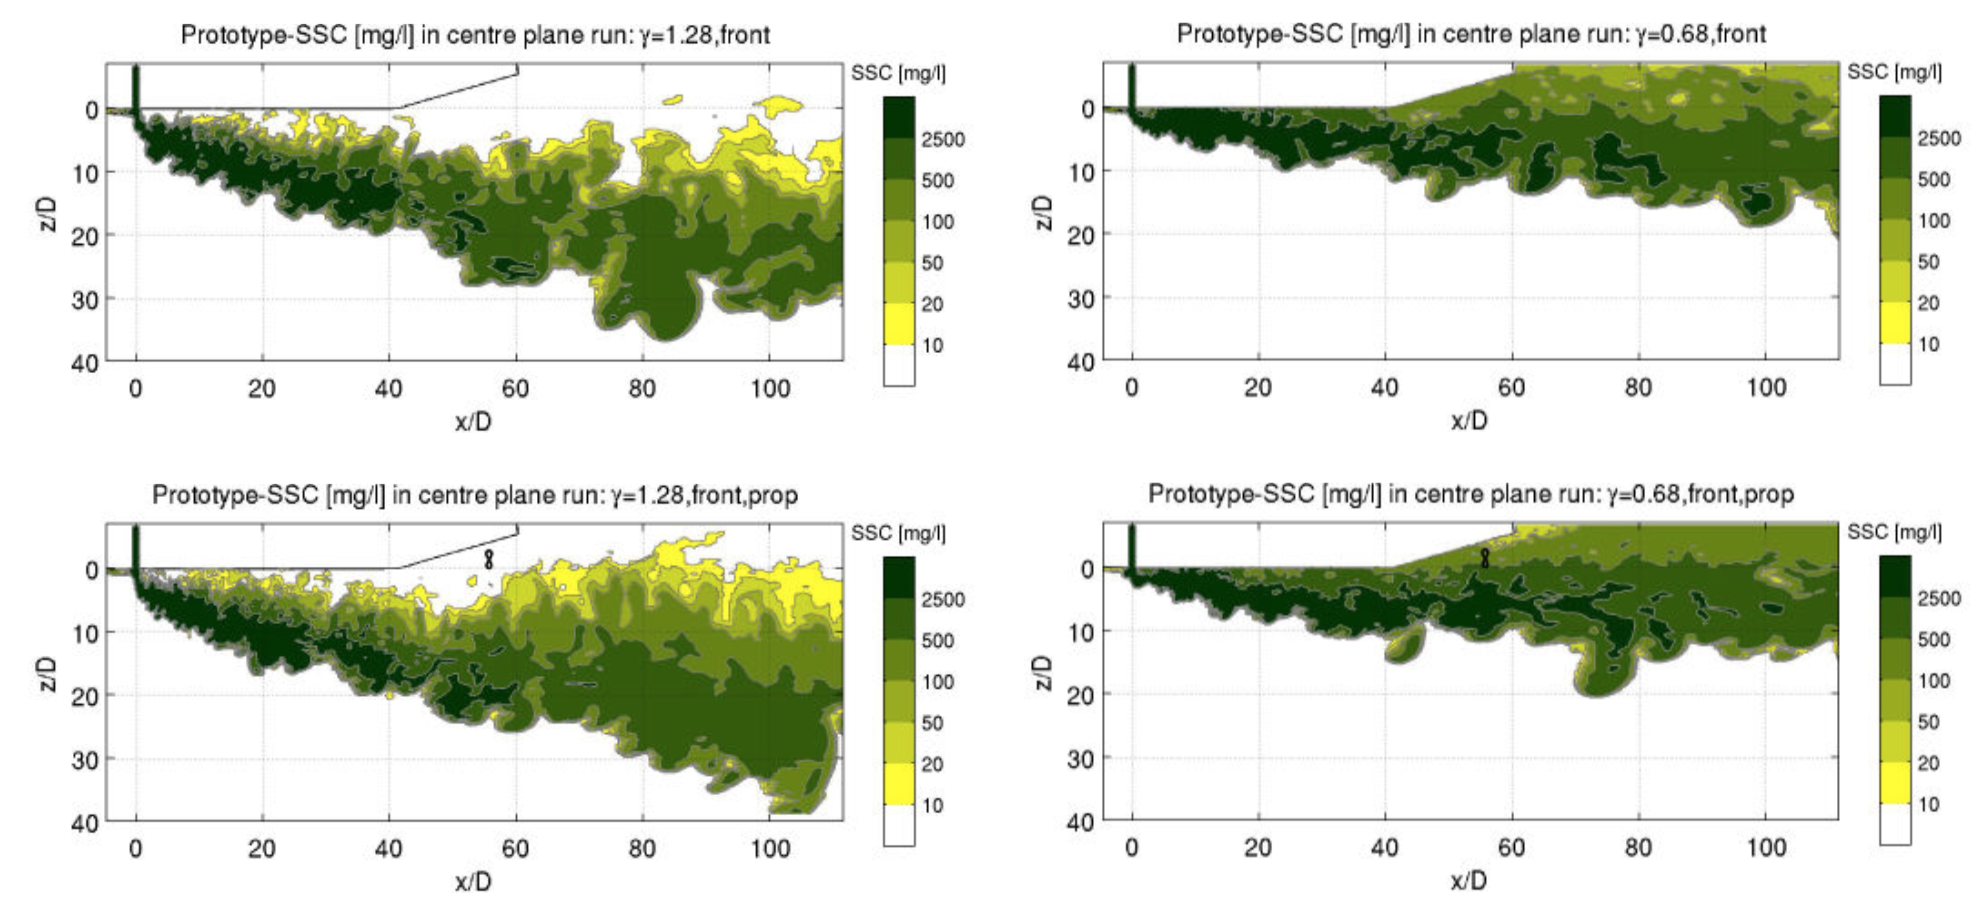
\includegraphics[width = 0.8\textwidth]{Images/Propeller_dewit.png}
    \caption{Influence of propeller with normal dredging speed (left) and high dredging speed (right)}
    \label{fig:Propeller_dewit}
\end{figure}

%







%%%%%%%%%%%%%%%%%%%%%%%%%%%%%%%%%%%%%%%%%%%%%%%%%%%%%%%%%%%%%%%%%%%%%%%%%%%%%%%%%%%%%%%%%%%%%%%%%%%%%%%%%%%%%%%%%%%%%%%%%%%%%%%%%%%%%%%%%%%%%%%%%%%%%%%%%%%%
\newpage
\section{Position of overflow}
\label{sec:position_overflow}
%belg 8.7.9
%De wit (105) + figuur 7.8
%two overflows (belg 8.7.10)

In section \ref{sec:propeller} is was shown that the propeller has influence in the vertical flux distribution of the plume. In addition to this, it can be argued that the distance from the overflow to the propeller could have influence. This will be further discussed in this section. \newline

\noindent Figure \ref{fig:Overflow_position} shows the SSC at x = 100D for normal- and high dredging speed and different locations of the overflow: 22.6D from the front of the TSHD (front) or the overflow at 50.4D from the front of the TSHD (back) \citep{Dewit}. As can be seen, without propeller the plume concentrations do not differ much with the overflow at the front or at the back (figure \ref{fig:Propeller_dewit}). With a propeller the plume has moved upward a little. This effect of the propeller is caused by entrainment into the propeller jet: the dredging plume is sucked upward by this entrainment and fine particles could follow this, depending on particle size diameter, but this is more complex due to hindered settling. When the overflow is at the back, the influence of the propeller is larger, because of the reduced distance between outflow of the dredging plume and the propeller. Figure \ref{fig:Overflow_position2} shows the effect in x direction on the plume of the overflow position. It can be concluded that the position of the overflow and effect of the propellers are in connection with each other. 

\begin{figure}[ht!]
    \centering
    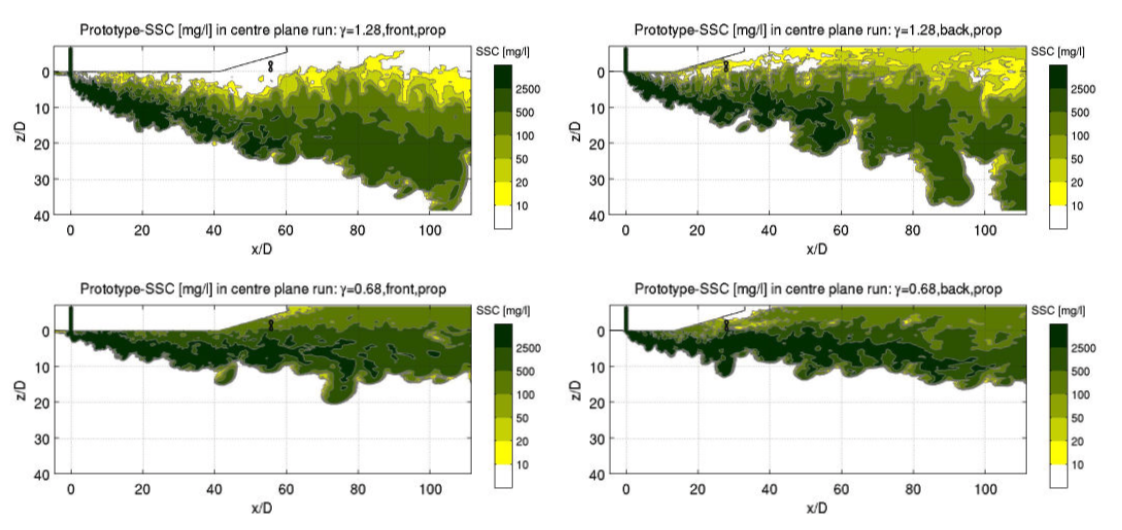
\includegraphics[width = 0.8\textwidth]{Images/Overflow_position_normal_high.png}
    \caption{Simulated instantaneous SSC at the centre slice for runs with normal dredging speed (top) and high dredging speed (bottom) with the overflow position in the front (left) and overflow position on the back (right)}
    \label{fig:Overflow_position2}
\end{figure}



\nomenclature[A]{$L_o$}{Distance from overflow to stern \nomunit{[$m$]}}
\nomenclature[A]{$B_o$}{Lateral distance from overflow to ships centerline \nomunit{[$m$]}}


\begin{figure}[H]
    \centering
    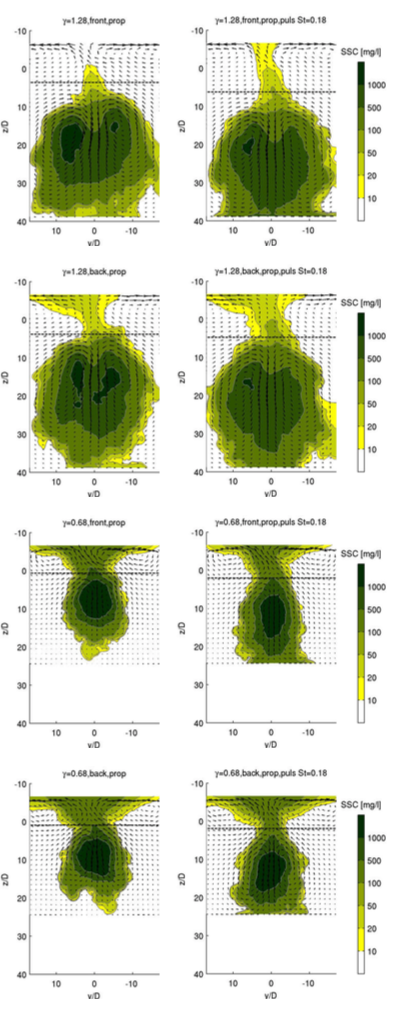
\includegraphics[width = 0.6\textwidth]{Images/Overflow_position.png}
    \caption{Simulated time averaged SSC at x =  100D of different runs with normal and high dredging speed. Arrows indicate the time averaged v, w velocity}
    \label{fig:Overflow_position}
\end{figure}

\noindent \cite{Decrop} used his LES model for the same investigation, however took the position of the overflow relative to the stern with the longitudinal distance between the overflow and stern ($L_o$) and lateral distance ($B_o$) to the ships centerline, which is shown in figure \ref{fig:Overflow_location}. Both the influence of $L_o$ and $B_o$ are investigated. In addition, a case with two overflows (one in the front and one in the back) is examined.

\begin{figure}[ht!]
    \centering
    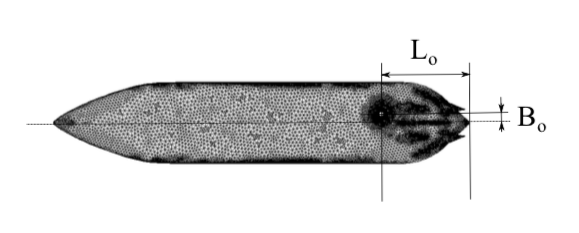
\includegraphics[width = 0.6\textwidth]{Images/Overflow_location_belg.png}
    \caption{Definition of longitudinal- and lateral overflow position $L_o$ and $B_o$}
    \label{fig:Overflow_location}
\end{figure}



\noindent Firstly, the influence of $L_o$ is investigated. It can be assumed that a longer distance $L_o$ is beneficial for the surface plume. When looking at the simulation results of \cite{Decrop} for a relatively horizontal plume (figure \ref{fig:Overflow_position_belg}) the longer distance $L_o$ seems to give the plume more time to detach from the keel and escape the propeller mixing. A smaller $L_o$ (figure \ref{fig:Overflow_position_belg}a) ensures the plume to be caught in the uplifting flow of the propeller and mixes the plume. The result is a much more uniform sediment distribution and a higher concentration in the surface plume.

\begin{figure}[ht!]
    \centering
    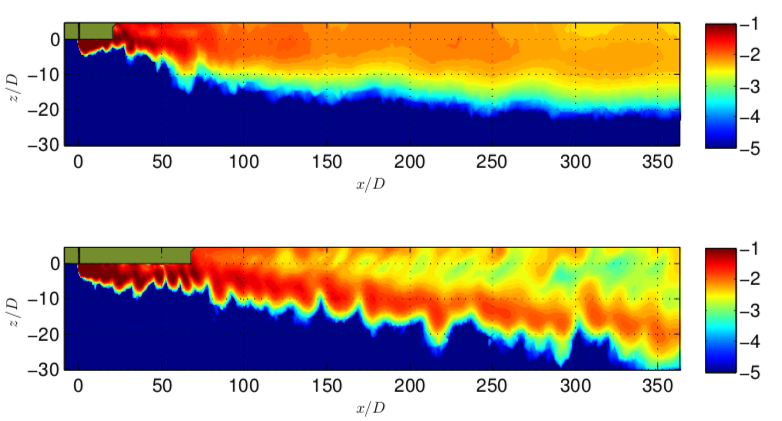
\includegraphics[width = 0.6\textwidth]{Images/Overflow_position_belg.png}
    \caption{Relative sediment concentration log($C$/$C_0$) at the symmetry plane, with H = 40m, $W_0$ = 3.2 m/s, $U_{cf}$ = 1.5 m/s, $C_0$ = 20 g/l and D = 1.1m. Overflow position $L_0$ differs: $L_o$ = 20m (a) and $L_o$ = 80m (b)}
    \label{fig:Overflow_position_belg}
\end{figure}


\noindent When looking at the results for a more dense plume with more rapid descent, the difference between smaller and longer $L_o$ is smaller, see figure \ref{fig:Overflow_position_belg_2}. Already after the short distance $L_o$ = 30m (figure \ref{fig:Overflow_position_belg_2}a), the plume has had the time to detach slightly from the hull. Therefore, the mixing of the propeller jet can just be avoided. The surface plume concentration is therefore only slightly higher compared to the case with $L_o$ = 80 m (figure \ref{fig:Overflow_position_belg_2}b). 

\begin{figure}[H]
    \centering
    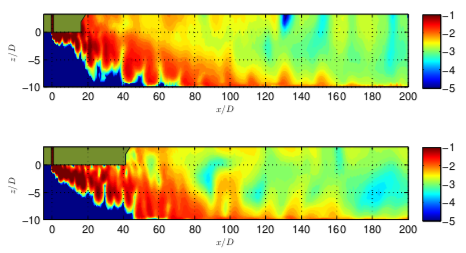
\includegraphics[width = 0.6\textwidth]{Images/Overflow_position_belg_2.png}
    \caption{Relative sediment concentration log($C$/$C_0$) at the symmetry plane, with H = 26 m, $W_0$ = 1.9 m/s, $U_{cf}$ = 2 m/s, $C_0$ = 90 g/l and D = 2 m. Overflow position $L_o$ differs: $L_o$ = 30 m (a) and $L_o$ = 80 m (b)}
    \label{fig:Overflow_position_belg_2}
\end{figure}


\noindent \textbf{Shift in lateral distance} \newline
\noindent In some vessels, an overflow is not located on the centerline of the vessel. The same case as in figure \ref{fig:Overflow_position_belg}a has been simulated with the overflow at $B_o$ = 5m from the centerline (figure \ref{fig:Overflow_position_Bo}). The effect of $B_o$ >0 depends on the geometry of the stern section and of $L_o$. In this case, the strongly curved hull sections near the stern and away from the ship’s centerline cause an uplifting flow, taking the plume upwards and causing an increased surface plume concentration. When the overflow is positioned at the centerline, these sloping parts are not encountered by the plume. At least in the geometry with which this model has been set up \citep{Decrop}.

\begin{figure}[ht!]
    \centering
    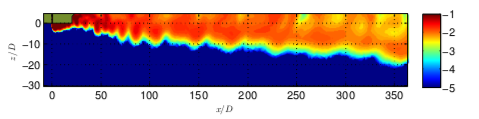
\includegraphics[width = 0.6\textwidth]{Images/Overflow_position_Bo.png}
    \caption{Relative sediment concentration log($C$/$C_0$) at the symmetry plane, boundary conditions same as in figure \ref{fig:Overflow_position_belg}, $L_o$ = 20 m. The lateral overflow position $B_o$ was changed to 5m instead of 0m}
    \label{fig:Overflow_position_Bo}
\end{figure}


\noindent \textbf{Two overflows} \newline
\noindent A case has been set up with the same boundary conditions as in figure \ref{fig:Overflow_position_belg}a. In that figure, two cases are shown. One with $L_o$ = 30m and one with $L_o$ = 80m. In the current case, the overflow discharge has been equally distributed over two overflows by halving the outflow velocity and keeping the same overflow diameter D and concentration $C_0$. The resulting vertical sediment profile at x/D = 100 is shown in figure \ref{fig:Multiple_overflows}. Despite to the lower exit velocity $W_0$, which should be a disadvantage, the plume with multiple overflows has a deeper average position and the overall concentrations are also lower. However, it can be observed (not shown) that due to the lower concentrations in the two overflows, more particles will be in suspension and is more diluted, which will increase the plume width \citep{Decrop}.

\begin{figure}[ht!]
    \centering
    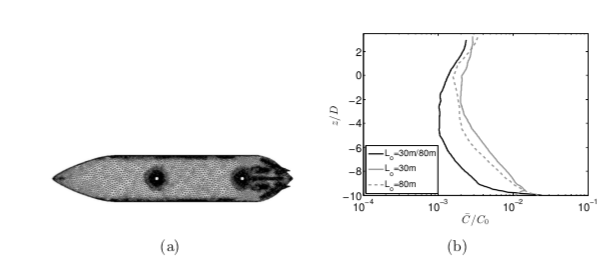
\includegraphics[width = 0.8\textwidth]{Images/Multiple_overflows.png}
    \caption{(a) Top view of the position of the two overflows in the vessel. (b) Profiles of time-averaged sediment concentration $C$/$C_0$ for three plume cases: $L_o$ = 30m/80m with two overflows and two cases with a single overflow at $L_o$ = 30m and 80m}
    \label{fig:Multiple_overflows}
\end{figure}






%%%%%%%%%%%%%%%%%%%%%%%%%%%%%%%%%%%%%%%%%%%%%%%%%%%%%%%%%%%%%%%%%%%%%%%%%%%%%%%%%%%%%%%%%%%%%%%%%%%%%%%%%%%%%%%%%%%%%%%%%%%%%%%%%%%%%%%%%%%%%%%%%%%%%%%%%%%%
\newpage
\section{Overflow sediment load}
%Belg 8.7.5

%Connectie met overflow position belg

The basic dimensionless numbers governing the behaviour of a buoyant jet were identified in section \ref{sec:froudenr} as the densimetric Froude number $F_{\Delta}$ and the velocity ratio $\lambda$. The sediment load in the overflow mixture, $C_0$, influences directly the Froude number $F_{\Delta}$. It is therefore expected that $C_0$ has an influence on the trajectory of near-field dredging plumes. \newline
\noindent \cite{Decrop} compared a total of eight cases with identical water depth H = 16m, $W_0$ = 1.9 m/s, $U_0$ = 1 m/s and D = 2m. The overflow was located at the front end of the hopper, at $L_o$ = 80 m from the stern. The two extremes are shown in figure \ref{fig:Sediment_load}, with $C_0$ = 10 g/l (top) and $C_0$ = 150 g/l (bottom). In these plots, the sediment concentration is shown, as before, as the relative value compared to $C_0$. Since in this case $C_0$ is varied this gives a distorted view. However, it is interesting to see that in the case of $C_0$ = 10 g/l the fraction of the initial sediment discharge ($C_0 Q_0$) present in the surface plume is about 100 times higher compared to the case with $C_0$ = 150 g/l. Evidently, in the field the absolute value of the sediment concentration is of importance. Yet, the question could be raised whether the total amount of sediment brought in suspension during a project could be reduced by releasing a more concentrated mixture. How this could be achieved in practise, is another question.

\begin{figure}[ht!]
    \centering
    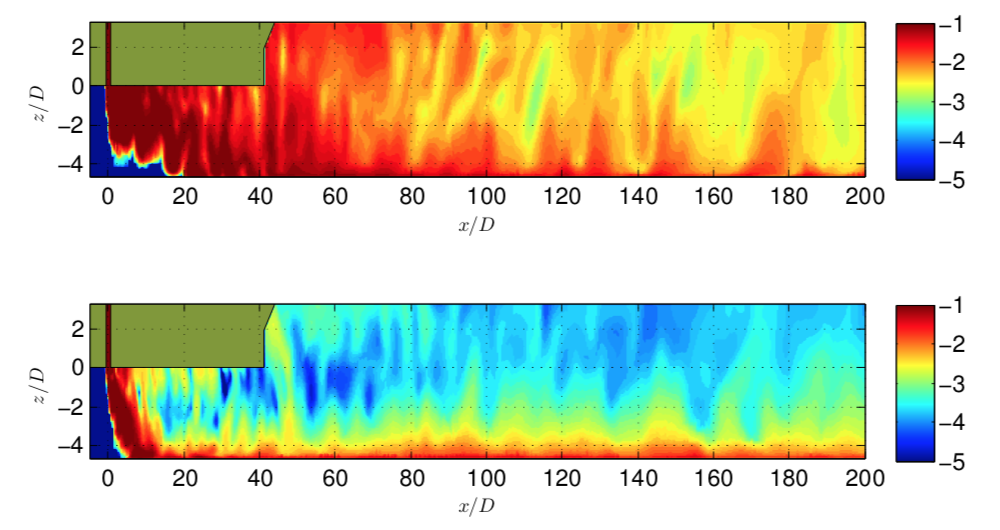
\includegraphics[width = 0.8\textwidth]{Images/Sediment_load.png}
    \caption{Relative sediment concentration log($C$/$C_0$) at the symmetry plane, with H = 16m, $W_0$ = 1.9 m/s, $U_0$ = 1 m/s, $L_o$ = 80m and D = 2m. The sediment concentration at the overflow was varied: $C_0$ = 10 g/l (top) and $C_0$ = 150 g/l (bottom)}
    \label{fig:Sediment_load}
\end{figure}

\noindent Nevertheless, it is needed to analyze the absolute time-averaged concentration C in the surface plume as a function of the release concentration $C_0$. In figure \ref{fig:Sediment_load_2}, the results for simulations with eight different values for $C_0$ are shown by \cite{Decrop}. In this figure, the absolute concentration in g/l is shown at 0.5 m below the water surface. It is surprising to see that very consistently, the sediment concentration in the surface plume decreases when the initial overflow concentration $C_0$ is increased. Between the stern at x/D = 40 and x/D = 120, the surface plume with $C_0$ = 10 g/l has sediment concentrations about twice as high as the plume with $C_0$ = 150 g/l. Further downstream, the difference becomes smaller, to about a factor 1.5. \newline

\begin{figure}[ht!]
    \centering
    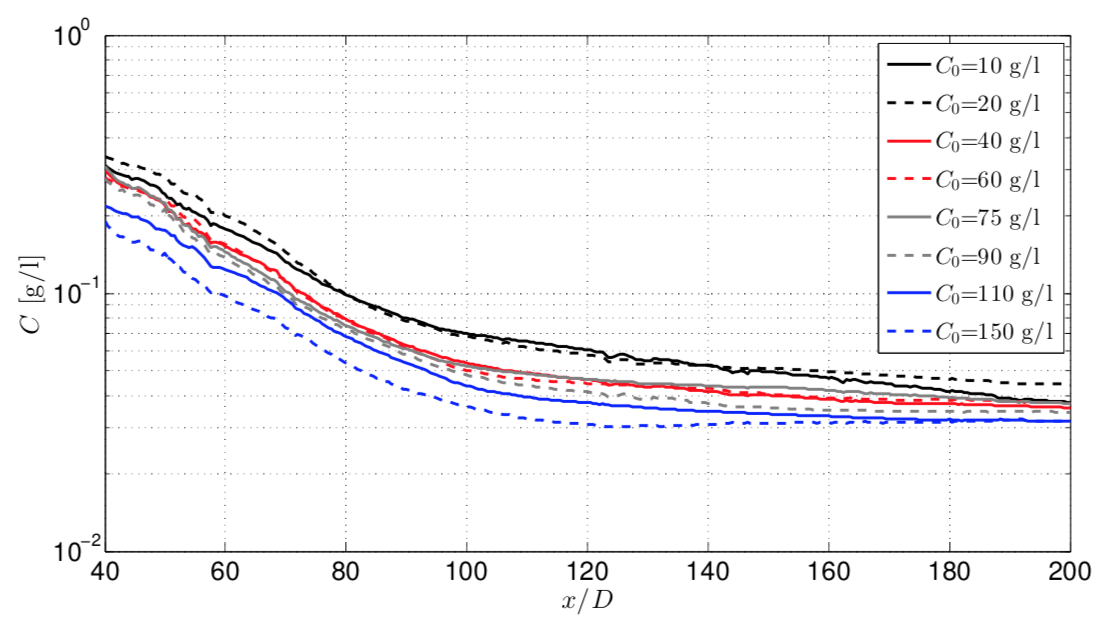
\includegraphics[width = 0.8\textwidth]{Images/Sediment_load_2.png}
    \caption{Comparison of absolute sediment concentration C as function of the initial overflow concentration $C_0$ at z = 0.5m}
    \label{fig:Sediment_load_2}
\end{figure}


\noindent This observation leads to the conclusion that releasing a more concentrated water-sediment mixture could significantly reduce the total amount of sediments brought in suspension.







%%%%%%%%%%%%%%%%%%%%%%%%%%%%%%%%%%%%%%%%%%%%%%%%%%%%%%%%%%%%%%%%%%%%%%%%%%%%%%%%%%%%%%%%%%%%%%%%%%%%%%%%%%%%%%%%%%%%%%%%%%%%%%%%%%%%%%%%%%%%%%%%%%%%%%%%%%%%

\section{Overflow outflow velocity}
%Dewit conclusie

A larger initial overflow velocity brings the overflow plume quicker to the bed, this increases the deposition in the near field and reduces the interaction between the plume and the TSHD hull and the plume and the TSHD propellers. However, an increased overflow velocity also means a larger overflow sediment source flux is brought into suspension \citep{Dewit}. Figure \ref{fig:Overflow_exit_velocity} shows the variation of the overflow exit velocity on $FF_{nf}$ and the vertical distribution (VIF) at x = 350m. It can be concluded that an increase of overflow outflow velocity does not show a large decrease of sediment flux in suspension at the end of the near field.


\begin{figure}[ht!]
    \centering
    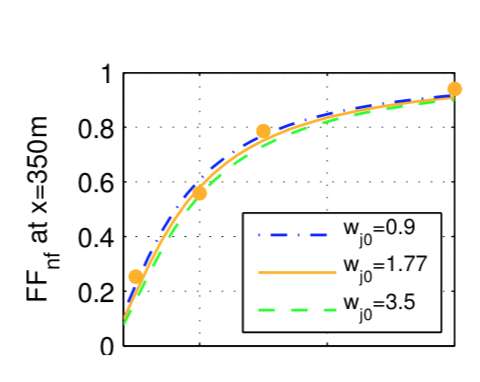
\includegraphics[width = 0.5\textwidth]{Images/Overflow_exit_velocity.png}
    \caption{Influence of overflow exit velocity ($w_{j0}$) at x = 350m}
    \label{fig:Overflow_exit_velocity}
\end{figure}

\noindent \cite{Boot} investigated the near-field spread of an overflow plume in an experimental setting. Three different densities ($\rho$ =  1016, 1033, 1049 $kg/m^3$) and three different outflow velocities ($U_{uitstr}$ =  0.05, 0.1, 0.2 m/s) are used, with a variable ambient flow velocity (6.5, 13 cm/s). With these inputs, \cite{Boot} determined if the outflow stayed a density current, became a transition current or a mixed current (see chapter \ref{sec:plume}) before it hits the bottom of the tank. It is shown, that the outflow velocity and density of the water-sediment mixture are correlated with each other. The increase in density leads to a shift to more density current profile but did not show large differences between the varying velocities with the 6.5 cm/s ambient current. Larger differences are noted when the ambient current increased to 13 cm/s, where all outflow velocities are in the transition zone or mixed flow in exception to $\rho$ =  1049 $kg/m^3$, $U_{uitstr}$ =  0.2 m/s, where it becomes a density current.\newline
\noindent However, in the experimental setup of \cite{Boot} the depth is limited and therefore outcomes can be different with larger depths in practice. Another limitation was the overflow diameter, which was fixed to 2.5cm in the model which should be 5cm to be more exact scaled in practice. In conclusion, the influence of different outflow velocities is limiting, depending on the ambient current. While a density current reaches deeper than a mixed current, it is not concluded in this experiment how deep it reaches compared with the other currents.




\nomenclature[A]{$U_{uitstr}$}{Outflow velocity from experiment by \cite{Boot} \nomunit{$[m/s]$}}


%%%%%%%%%%%%%%%%%%%%%%%%%%%%%%%%%%%%%%%%%%%%%%%%%%%%%%%%%%%%%%%%%%%%%%%%%%%%%%%%%%%%%%%%%%%%%%%%%%%%%%%%%%%%%%%%%%%%%%%%%%%%%%%%%%%%%%%%%%%%%%%%%%%%%%%%%%%%

\section{Overflow shape}
\label{sec:shape}
%Belg (259)

Different studies have shown that non-circular shapes of exit holes of buoyant jets in cross flows have an impact on the jet trajectory. \cite{Salewski+} found that an elliptical jet exit with aspect ratio of 1.69 had a 10\% better penetration in the cross flow compared to a circular hole with the same surface area (at x/D = 10). \cite{Haven+} also showed that high-aspect ratio openings enhance the cross flow penetration. \newline
\noindent These findings lead to the question whether an overflow opening with higher aspect ratio could improve the plume outflow from the TSHD keel wall. \cite{Decrop} simulated  two test cases with a rectangular overflow cross section. The surface area of the rectangular cases was identical to the reference cases with D = 2m shafts. The rectangular shafts were 3m in length (along ship axis) and $\pi$/3m in width. The aspect ratio of the rectangular overflow shaft is therefore equal to $\pi$. All other conditions were kept constant.

\begin{figure}[ht!]
    \centering
    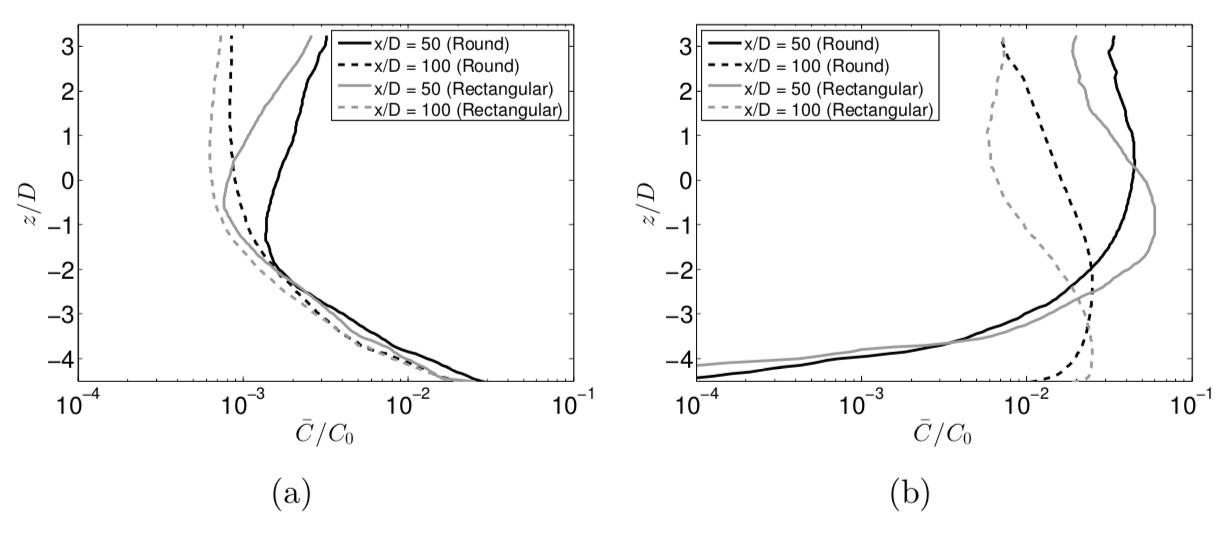
\includegraphics[width = 0.8\textwidth]{Images/Overflow_shape.png}
    \caption{Time-averaged sediment concentration $C/C_0$, for 2 cases in which a round overflow shaft was compared with a rectangular shape with high aspect ratio. For both shapes the cross-sectional area of the overflow shaft was equal to $\pi$. In (a), $U_0$ = 1 m/s, $C_0$ = 55 g/l and $W_0$ = 1.9 m/s. In (b) $U_0$ was increased to 3 m/s}
    \label{fig:Overflow_shape}
\end{figure}

\noindent A first case with $U_0$ = 1 m/s, $C_0$ = 55 g/l and $W_0$ = 1.9 m/s was investigated by \cite{Decrop}(figure \ref{fig:Overflow_shape}a). This case is clearly of type density current with a distinct surface plume. With a round overflow shaft, the sediment concentrations in the upper half of the water column are about 25\% to 50\% higher compared to the case with rectangular overflow. It seems that the shape of the overflow shaft does have an influence in the lower half of the water column. Either the higher aspect ratio in the rectangular case leads to a better escape from the keel, or the more narrow shape of the plume after exit might reduce the number of air bubbles that escape per unit of time, leading to less surface plume generation in the first few meters after the exit.\newline
\noindent In the second case, the cross flow velocity was increased to $U_0$ = 3 m/s. It is determined in this test case whether a high-aspect ratio overflow shaft would lead to a reduction of the surface plume concentration. The result of the simulations of this case with round (D = 2m) and equivalent rectangular shape is shown in figure \ref{fig:Overflow_shape}b. At x/D = 50, it can clearly be observed that the bulk of the plume is situated lower for the rectangular case compared to the round shaft. The surface concentration is 40\% lower in the rectangular case. After x/D = 100, the difference in concentration near the surface has reduced, but it is clear that less sediments are present in the water column in the near-field overflow plume.\newline
\noindent The influence of the shape of the overflow shaft needs more investigation to draw definite conclusions, but it seems that variations in the aspect ratio of the shaft cross section have the potential to reduce the sediments in suspension in the overflow plume. \newline

\noindent In another vision, \cite{Wang} looked at the heat transfer and flow through an elliptic duct and the effect of roundness of the corners with different aspect ratios. The curves are noted with n, which is shown in figure \ref{fig:elliptic_shapes} where c is noted as the aspect ratio (2L is the length of the major axis and 2cL is the length of the minor axis (0 < c $\leq$ 1)). A curve with n=$\infty$ approaches the values of a rectangular duct and a curve with n=$\infty$ and c=1 approaches the values of a square duct.

\begin{figure}[ht!]
    \centering
    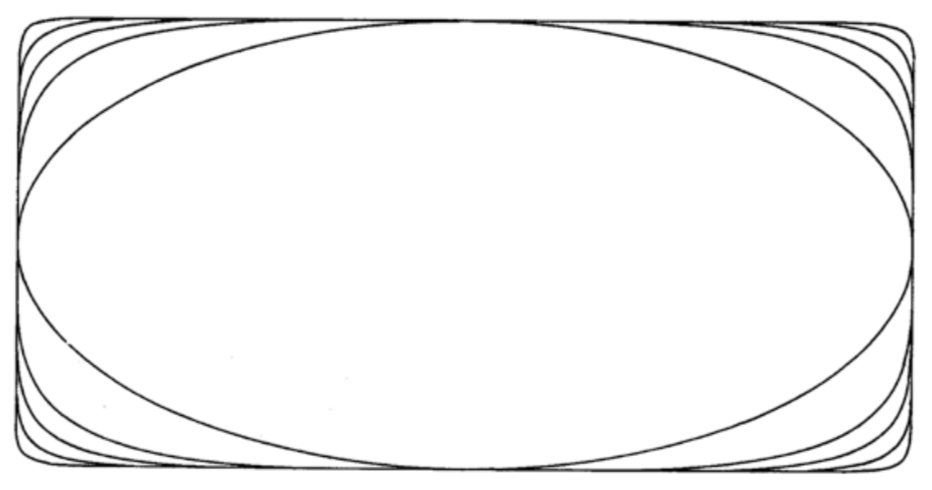
\includegraphics[width=0.5\textwidth]{Images/Elliptic_shapes.png}
    \caption{Super-elliptic cross sections for aspect ratio c = 0.5. Curves from inside: n = 1, 2, 3, 5, 10}
    \label{fig:elliptic_shapes}
\end{figure}

\nomenclature[G]{$\sigma_m$}{Normalized minimum wall shear stress \nomunit{[-]}}
\nomenclature[A]{$c$}{Aspect ratio \nomunit{[-]}}

\noindent The interest of corner rounding is shown by the minimum shear stress ($\sigma_m$) near a rounded corner. As said, with n=$\infty$ the curve approaches the values of a rectangular duct where $\sigma_n$=0 near the corners. The values of $\sigma_n$ with different values of n and c are shown in figure \ref{fig:shapes_table}. Here \cite{Wang} compared different n values with four cases from left to right (c=1, c=0.75, c=0.5, c=0.25).


\begin{figure}[ht!]
    \centering
    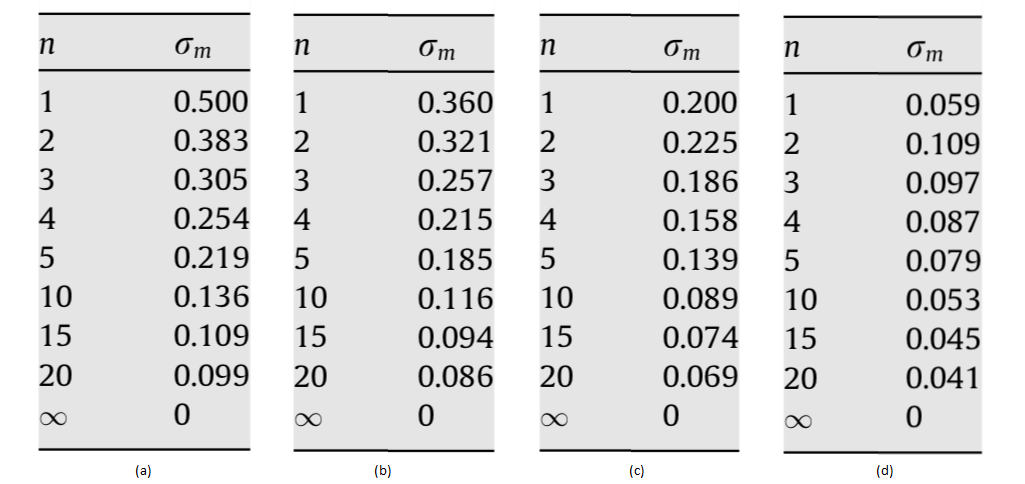
\includegraphics[width=0.8\textwidth]{Images/n_sigma_m.png}
    \caption{Properties of a duct with aspect ratio (a) c=1, (b) c=0.75, (c) c=0.5, (d) c=0.25}
    \label{fig:shapes_table}
\end{figure}


\noindent It is concluded that a rectangular shape with a high aspect ratio (low value of c) shows a decrease in shear stress near the rounded corners ($\sigma_m$) which connects to the founding of \cite{Decrop}.










%%%%%%%%%%%%%%%%%%%%%%%%%%%%%%%%%%%%%%%%%%%%%%%%%%%%%%%%%%%%%%%%%%%%%%%%%%%%%%%%%%%%%%%%%%%%%%%%%%%%%%%%%%%%%%%%%%%%%%%%%%%%%%%%%%%%%%%%%%%%%%%%%%%%%%%%%%%%
\newpage
\section{Extension of overflow}
\label{sec:extension}
%\textbf{Extension of overflow (262) + PHD verslag de wit}

As shown earlier, the water depth and propeller have influence on the plume dispersion while dredging. Both \cite{Dewit} and \cite{Decrop} investigated therefore an extension of the overflow to bring the outflow of the overflow deeper, so bring the sediment closer to the bed, and reduce impact of the propeller. \newline

\noindent \cite{Dewit} investigated three overflow extensions for dredging in a depth of 25m:
\begin{itemize}
    \item Short extension of 3m long
    \item Medium long extension of 8m long
    \item Long extension of 16m long (1m above seabed) 
\end{itemize}

\noindent \cite{Dewit} compared the extensions with a base run (no extension) with following parameters: $\rho_{outflow}$ =  1200 $kg/m^3$, 4 \% air with $T_p$ =  5.5s, $W_0$ =  1.77 m/s, D =  2.25m, depth =  25m, draft =  8m, $\rho_{ambient}$ =  1300 $kg/m^3$. For computational reasons, the overflow shape was square of 2.5m internally. In extension, the 16m overflow was computed to have a horizontal outflow instead of vertical. In order to investigate the interaction between the influence of the THSD sloping aft and propellers, \cite{Dewit} tested two locations: 100m- and 40m in front of the TSHD aft. Figure \ref{fig:Overflow_extension_dewit} shows the suspended sediment concentration for the three overflow extensions.


\begin{figure}[ht!]
    \centering
    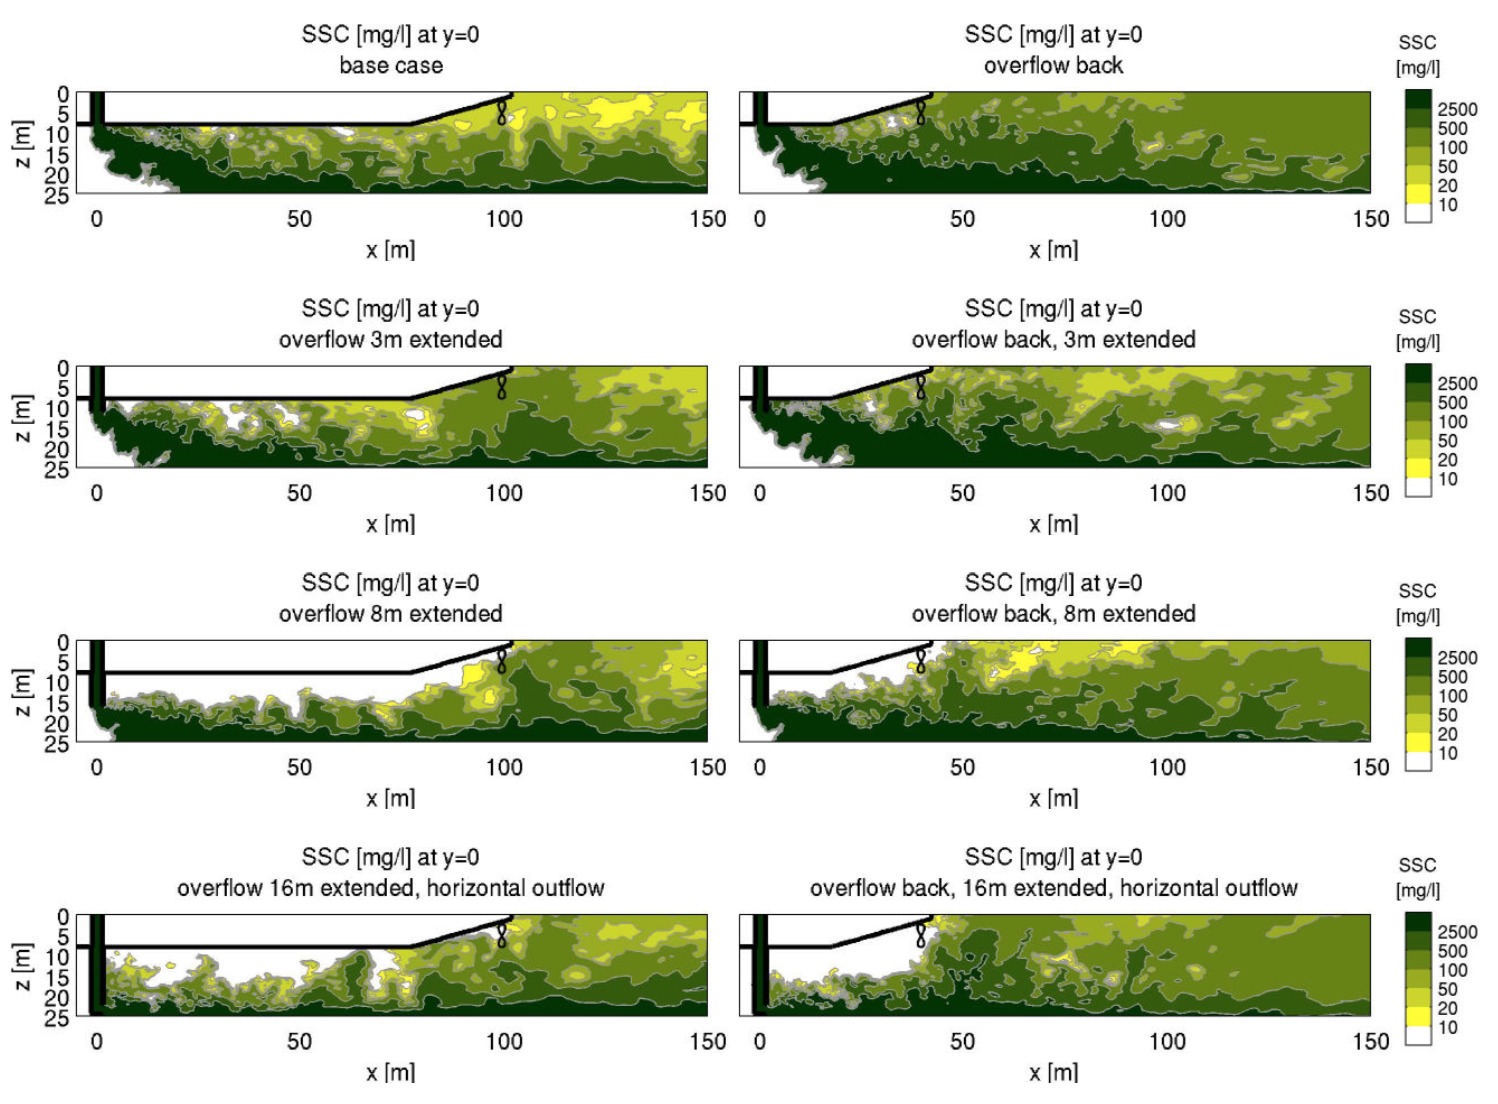
\includegraphics[width = 1\textwidth]{Images/Overflow_extension_dewit.png}
    \caption{SSC at y = 0 for different overflow extensions}
    \label{fig:Overflow_extension_dewit}
\end{figure}

\noindent In the base case, without an overflow extension, the plume spreads over the complete zone below the keel and suspended sediment clouds of SSC > 100 mg/l touch the keel. A 3m extended overflow has limited influence on the instantaneous SSC distribution at y = 0, but a 8m extension results in a zone free of suspended sediment below the keel of the TSHD. The 16m overflow extension brings the sediment right at the bed without mixing, but then the sediment is re-suspended up in the water column by the air fraction from the overflow mixture and the turbulent interaction between the vertical overflow extension and the cross flow. This re-suspension is so strong that some puffs of suspended sediment reach the keel of the TSHD before the sloping aft of the TSHD. The re-suspension caused by air of the 16m overflow extension is larger than the re-suspension by air of the 3m and 8m extensions as the outflow of the 3m and 8m extensions. These two extensions have downward momentum leading to more separation of the air from the sediment-water mixture than with the 16m extension which has horizontal outflow.\newline 
\noindent At the sloping aft, the flow expansion and entrainment into the propeller jet even brings suspended sediment to the free surface. With the overflow at the back the plume spreads more in vertical direction and larger SSC values are found at the free surface than with the overflow at the front. This holds for all cases, with and without overflow extension, and is caused by the shorter distance from the overflow to the TSHD aft and propellers. \newline

\noindent \cite{Decrop} made a case with the LES model to verify the findings of \cite{Dewit}. In addition, the overflow was positioned near the stern of the ship, with a lateral shift of $B_o$ =  4m. In section \ref{sec:position_overflow} it was shown that a lateral shift, and an overflow in the back, were both unfavourable for the creation of surface plumes. \cite{Decrop} compared two overflow extensions (3m, 5m) with a base case with the following parameters: H =  40m, $W_0$ =  3.2 m/s, $U_cf$ =  1.5 m/s, D=1.1m and $C_0$ =  20 g/l. Figure \ref{fig:Overflow_extension_belg} displays the relative sediment concentration at the symmetry plane of $B_0$ =  4m.


\begin{figure}[ht!]
    \centering
    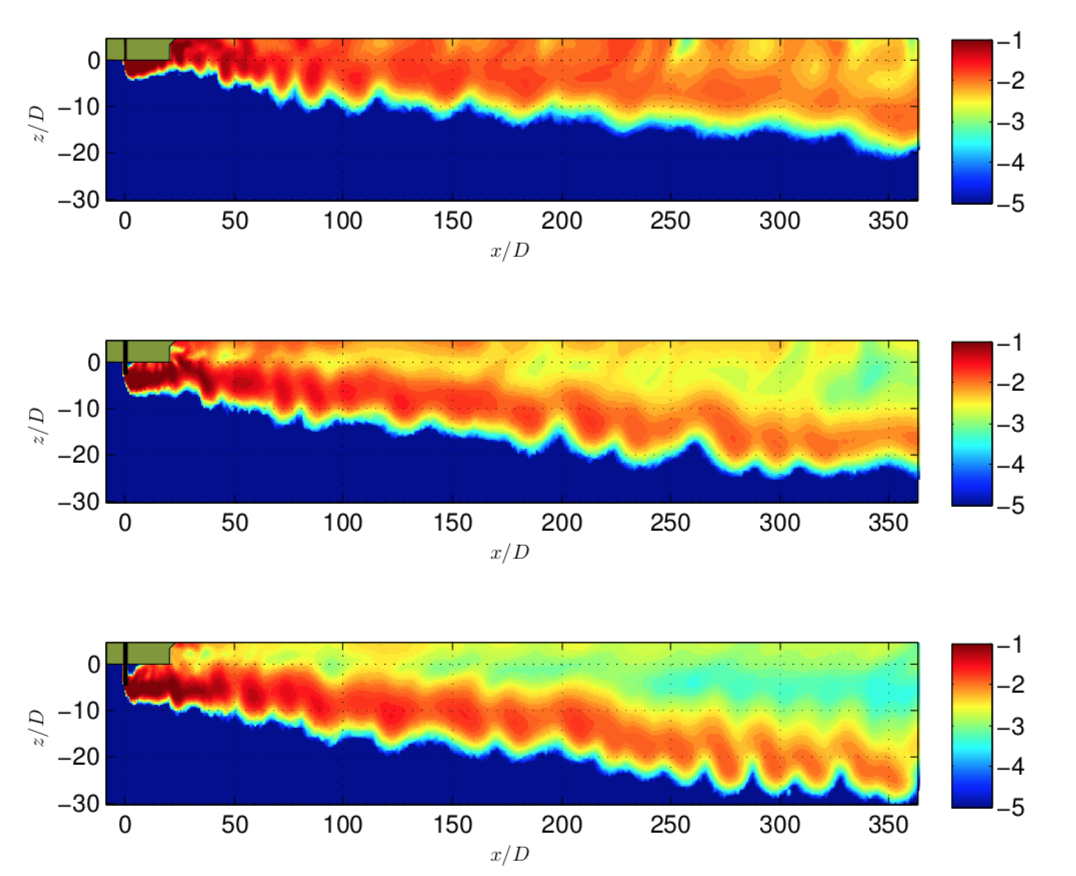
\includegraphics[width = 0.8\textwidth]{Images/Overflow_extension_belg.png}
    \caption{Relative sediment concentration log($C/C_0$) at $B_0$ =  4m with overflow extension =  0m (top), 3m (middle), 5m (bottom)}
    \label{fig:Overflow_extension_belg}
\end{figure}

\noindent It can clearly be observed that in the case with no extension, the overflow plume moves completely to the surface (top panel). With an extension length of 3m, the main plume is allowed to escape the uplifting effect of the curved stern sections, but a relatively high sediment concentration remains present in a surface plume (middle panel). This can be explained by the fact that the plume was not deep enough to escape the propeller jet. For an extension length of 5m, the plume escapes both the uplifting of the stern and the propeller jet mixing (bottom panel). The main plume descends steadily towards the sea bed. Air bubbles still have an influence, which cannot be avoided unless an over
overflow extension is combined, for example, with an environmental valve. However, it is noted that an environmental valve is inefficient with an lateral shift of the overflow \citep{Decrop}. It can be seen that even in the case with an overflow length of 5m, some sediment is torn off above the plume right after the exit, due to air bubble entrainment. \newline

\noindent Additionally, \cite{Decrop} made an overview of the vertical $C/C_0$ profiles (figure \ref{fig:Overflow_extension_belg_2}) for different extension lengths and two distances behind the dredger.


\begin{figure}[ht!]
    \centering
    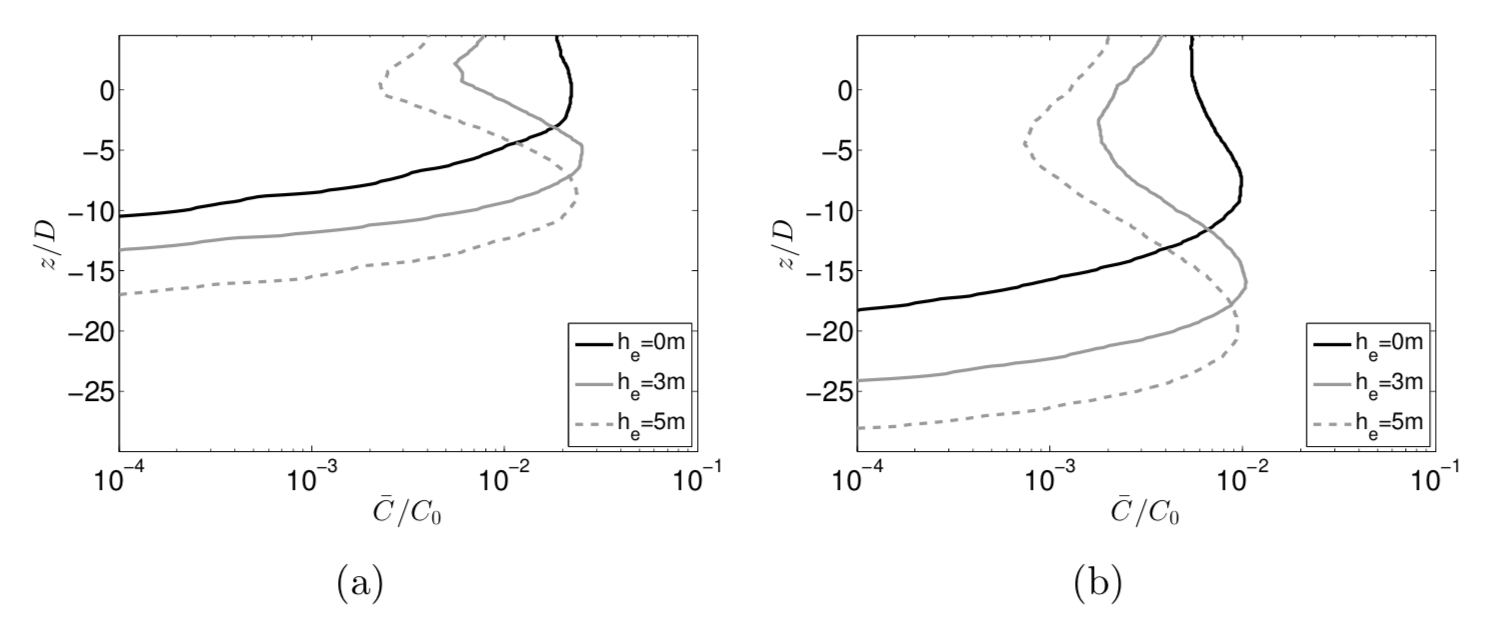
\includegraphics[width = 1\textwidth]{Images/Overflow_extension_belg_2.png}
    \caption{Vertical profiles of time-averaged sediment concentration $C/C_0$}
    \label{fig:Overflow_extension_belg_2}
\end{figure}

\noindent Figure \ref{fig:Overflow_extension_belg_2}a shows the profiles at x/D=100. It can be observed that the maximum concentration in the plumes remains similar, but that the plume center is deeper for longer extension lengths. The difference between the depth of the concentration (at $10^{-4}$ in figure \ref{fig:Overflow_extension_belg_2}), for extension lengths 3m and 5m is larger then the difference in extension length (2m). More important is the fact that the surface concentration decreases a factor 2.5 with a 3m extension and a factor 5 with a 5m extension. When looking further downstream (x/D=300; figure \ref{fig:Overflow_extension_belg_2}b), the same pattern is found, where plumes with increasing extension are deeper and have a lower surface concentration. The surface plume reductions at x/D=300 are smaller, but still noticeable. \newline

\noindent The extension, as showed, has noticeable positive effects on the surface plume. However, an overflow extension will create a extra torque around the point where the extension is connected to the hull. In addition, the extended overflow pipe will have strong interaction with the ambient flow, which creates a different flow pattern. 







%%%%%%%%%%%%%%%%%%%%%%%%%%%%%%%%%%%%%%%%%%%%%%%%%%%%%%%%%%%%%%%%%%%%%%%%%%%%%%%%%%%%%%%%%%%%%%%%%%%%%%%%%%%%%%%%%%%%%%%%%%%%%%%%%%%%%%%%%%%%%%%%%%%%%%%%%%%%
%TABEL MET OPSOMMING VAN ELKE FACTOR VOOR EN NADELEN ETC.
%grootste factoren volgens belg en de wit
%MCA en keuze welke factor aanpakken

\newpage
\section{Conclusion}
\nomenclature[Z]{MCA}{Multi Criteria Analysis}


In the past paragraphs, twelve factors are investigated to decrease the surface turbidity of overflow losses on a TSHD. In order to get a good overview, which factors are the most promising to investigate further into an practical solution, the factors are divided in three parts: A recommendation- , no influence- or a further investigation part. A multi-criteria-analysis is done to conclude which factor is the most promising solvable factor that will be further investigated into a practical solution. In this MCA questions like, is a solution practical possible? or is it economic feasible? will be answered. First all factors are showed in an overview (Table \ref{tab:Overview_factors}) with a short conclusion. \newline 

\begin{table}[ht!]
\centering
\caption{Overview contributing factors which lead to surface turbidity , with their conclusions}
\label{tab:Overview_factors}
\begin{adjustbox}{max width=\textwidth}
\begin{tabular}{|l|l|}
\hline
\textbf{Factor}                        & \textbf{Conclusion}                                                                                                                                                                                                                                                                                                                                                                   \\ \hline
Hopper inlet / sedimentation           & Change the filling process to decrease overflow losses in the last phase, where these increase exponentially                                                                                                                                                                                                                                                            \\ \hline
Dredging speed                         & \begin{tabular}[c]{@{}l@{}}An increase of $U_{cf}$ of 3, will increase the surface plume concentration $C/C_0$ 10 times at X/D = 100 \\ Horizontal spreading is decreased with a higher dreding speed\end{tabular}                                                                                                                                                                    \\ \hline
Dredging / water depth                 & \begin{tabular}[c]{@{}l@{}}A keel clearance of \textgreater 9m will not decrease the surface plume concentration more\\ An increase from $H_k$ = 5m to $H_k$ = 9m increases the surface streamwise velocity around a factor 1.3\\ An increase of water depth will increase the amount of flux near the bed\end{tabular}                                                               \\ \hline
Angle between TSHD \& ambient current & \begin{tabular}[c]{@{}l@{}}Due to the angle, surface plume is diverted\\ Total sediment flux is quite similar compared without cross flow \\ More interaction with hull and propeller, leads to upward flow to surface\end{tabular}                                                                                                                                                                                                                                \\ \hline
Pulsing                                & \begin{tabular}[c]{@{}l@{}}Pulsing correlated with air entrainment, increase in pulsing will increase air entrainment\\ Increase in pulsing period ($T_p$) will increase surface plume\\ Pulsing period does not have large effect with a high dredging speed\end{tabular}                                                                                                            \\ \hline
Air                                    & \begin{tabular}[c]{@{}l@{}}Entrained air will follow a other path than the water-sediment mixture\\ Air will release to the surface after outflow of the overflow and could take fine particles with it\\ 12\% air with $T_p$ = 5.5s will increase the surface plume concentration with 200 mg/l and\\ spreads the surface plume with 100m compared to case with 0\%\end{tabular}     \\ \hline
Interaction with propeller             & \begin{tabular}[c]{@{}l@{}}Tangential component of propeller is 90\% dissipated at 4D\\ Almost no influence at high dredging speed\\ Lifts the plume from 20 mg/l (no propeller) to 50 mg/l at normal dreding speed at propeller height\\ A propeller was found to have more influence than overflow location and pulsing on the formation of a \\surface plume\end{tabular}                                                                                                                                  \\ \hline
Position of overflow                   & \begin{tabular}[c]{@{}l@{}}Position in the front of TSHD will decrease surface plume\\ Correlated with propeller, more is sucked in if overflow is at the back\\ Lateral shift of overflow will increase the surface plume\\ Multiple overflows (front and back) has deeper average position of plume and overall concentrations are \\ lower, plume width will increase\end{tabular} \\ \hline
Overflow sediment load                 & \begin{tabular}[c]{@{}l@{}}Absolute sediment concentrations will decrease with a factor 2 near the TSHD (40 \textless x/D \textless 120) and with \\ a factor 1.5 when increasing the overflow sediment load from $C_0$ = 10 g/l to $C_0$ = 150 g/l\\ from x/D \textgreater 120 when increasing the overflow sediment load from $C_0$ = 10 g/l to $C_0$ = 150 g/l\end{tabular}        \\ \hline
Overflow outflow velocity              & Overflow outflow velocity does not show a large decrease of sediment flux in suspension at end of near field                                                                                                                                                                                                                                                                          \\ \hline
Overflow shape                         & \begin{tabular}[c]{@{}l@{}}Rectangular shape will decrease sediment concentration in upper water column with 25-50\% in normal speed\\ Rectangular shape will decrease sediment concentration in upper water column with 40\% in high speed with\\ aspect ratio of $\pi$\end{tabular}                                                                      \\ \hline
Extension of overflow                  & \begin{tabular}[c]{@{}l@{}}Extension of overflow will bring plume deeper, but creates more re-suspesion because of air\\ Surface concentration decreases with factor 2.5 with 3m extension\\ Surface concentration decreases with factor 5 with 5m extension\end{tabular}                                                                                                             \\ \hline
\end{tabular}
\end{adjustbox}
\end{table}


\noindent Directly, the twelve factors can be divided in divided in three parts, where one part are more recommendations, other need further investigation to determine the amount of surface plume created and the last concluded to have more or less no influence on the creation of a surface plume. A good example is the dredging speed, which will be recommended to keep low. Table \ref{tab:Overview_factors} showed a 10 times increase in surface plum if the dredging speed is increased with a factor 3. The twelve factors are divided in these two parts and are shown in table \ref{tab:Part_factors}. In addition, all factors are described further why they are placed in a certain group.



\begin{table}[ht!]
\centering
\caption{Overview of splitting all factors in three parts: recommendation, no influence or further investigation}
\label{tab:Part_factors}
\begin{tabular}{|l|l|l|}
\hline
\textbf{Recommendations}              & \textbf{No Influence}      & \textbf{Further Investigation} \\ \hline
Dredging / water depth                & Overflow outflow velocity  & Hopper inlet / sedimentation   \\ \hline
Dredging speed                        & Interaction with propeller & Pulsing / Air                  \\ \hline
Position of overflow                  &                            & Overflow sediment load         \\ \hline
Angle between TSHD \& ambient current &                            & Overflow shape                 \\ \hline
                                      &                            & Overflow extension             \\ \hline
\end{tabular}
\end{table}



\newpage
\begin{itemize}
    \item \textbf{Hopper inlet / sedimentation} [\textit{Further investigation}]: The amount of surface plume is directly related to the amount of concentration in the overflow. A way to decrease the overflow loss in the hopper must be further investigated.
    \item \textbf{Dredging speed} [\textit{Recommendation}]: It is recommended that the dredging speed stays at normal level. Increase to higher dredging speed will exponentially increase the surface plume.
    \item \textbf{Dredging / water depth} [\textit{Recommendation}]: It is recommended that the water depth is larger than 9m. A water depth <9m will increase the surface plume and streamwise velocity. 
    \item \textbf{Angle between TSHD \& ambient current} [\textit{Recommendation}]: The total sediment flux is quite similar compared without a cross flow, only the plume is diverted. However, interaction with hull can be expected with higher angles, where sediment particles can be taken along by the expanding flow towards the free surface. Recommended to keep angle between TSHD and ambient current low.
    \item \textbf{Air / pulsing} [\textit{Further investigation}]: Air and pulsing are closely correlated because pulsing causes the inlet of air in the overflow. A solution which decreases the amount of entrapped air or pulsing must be investigated further.
    \item \textbf{Interaction with propeller} [\textit{No influence}]: A propeller does have influence on the surface plume due to the suction force by the propeller. However, a TSHD needs a propeller and therefore this is not further investigated.
    \item \textbf{Position of overflow} [\textit{Recommendation}]: A overflow that is positioned in the front of the TSHD will decrease surface plume because less interaction with the propeller. In addition, two overflows (front and back) will bring plume deeper.
    \item \textbf{Overflow sediment load} [\textit{Further investigation}]: Absolute sediment concentration will decrease with factor 2 near TSHD and with a factor 1.5 further away when increasing the overflow sediment load from $C_0$ = 10 g/l to $C_0$ = 150 g/l. Further investigation is needed to show if it is practical possible.
    \item \textbf{Overflow outflow velocity} [\textit{No influence}]: A change in overflow outflow velocity did not show a large decrease of sediment flux in suspension, so it is not further investigated.
    \item \textbf{Overflow shape} [\textit{Further investigation}]: A rectangular overflow shape showed a strong decrease of surface plume and so must be further investigated.
    \item \textbf{Overflow extension} [\textit{Further investigation}]: A overflow extension of >3m showed a strong amount of decrease in surface concentration and so must be further investigated.
\end{itemize} 


%Alle grafiek waardes weten!!! Decrop deWit

%milieu eisen dredging Australie bijvoorbeeld 

%korrelgrootte



